\chapter{Results}
\label{chapter:Results}
\section{Singleton opinion spam detection}

\setkeys{Gin}{width=0.8\textwidth} 


As mentioned in the \nameref{chapter:Method} chapter, I have used two clustering algorithms DBSCAN and OPTICS to create review groups based on the behavioral features. The purpose was to see which algorithm performs best on my dataset and better adapts to the user behavior. 
I have experimented with \textit{epsilon} in \{0.02, 0.05, 0.08, 0.1, 0.4\}. The two marginal values 0.02 and 0.4 produced very high clustering noise, meaning a lot of reviews were not clustered. They also recorded a very low precision and F1 score, so I will not mention them in this section.

Moreover, I have experimented with the cosine similarity including all words (excluding stopwords) and used nouns, verbs and adjectives parts-of-speech for the rest of the measures. The best results were obtained in the following scenarios:
\begin{itemize}
\item cosine similarity with all parts-of-speech tags, excluding stopwords
\item cosine similarity with non-lemmatized POSs - nouns, verbs and adjectives, excluding stopwords
\item cosine similarity with lemmatized POSs - nouns, verbs and adjectives, excluding stopwords
\item mihalcea semantic similarity - nouns, verbs and adjectives, excluding stopwords
\item maxsim - maximum value among of all the previous measures
\end{itemize}
Each candidate review pair compared was labeled as deceptive if it exceeded a certain similarity threshold. The minimum threshold value was set to 0.5 and the maximum value was 1, where 1 would indicate an identical pair of reviews.

The clustering phase managed to produce relevant clusters, although it was based on very simple behavioral features. It also produced a significant amount of noise. For DBSCAN with \textit{epsilon} = 0.1, the classifier performed very well, reaching even precision of over 90\% for higher thresholds. But a very large number of reviews was actually discarded from the similarity model because they were not clustered.

A conclusion would be that very dense review clusters are likely to be the result of a bursty behavior of a user which posts reviews for the same seller in a very short amount of time. This is a very obvious type of opinion spam, when the user usually also copy-pastes a large portion of the text between reviews. Upon manual inspection of the reviews in the clusters leading to such high precision, I could verify the reviews were indeed close to identical.

The DBSCAN approach offered good results using the cluster validation strategy. For \textit{epsilon} = 0.1 and minPts = 2, it achieved a precision of  90\% at thresholds larger than 0.85 for all the similarity measures, as Figure \ref{fig:dbscan-minpts-2-eps-0-1-precision-cluster} shows. The results were even better when the individual validation strategy was applied and the precision reached 90\% even with a threshold of 0.75 as Figure \ref{fig:dbscan-minpts-2-eps-0-1-precision-individual} shows. It can be observed that the precision of the semantic measure is generally very close or higher than that of the vectorial measures above a threshold of 0.7. The intuition that the scores should become more precise as the threshold is raised is proven by the results. Also in a production system, the threshold value can easily be tuned to achieve a desired precision.

The noise produced by DBSCAN was around 30\% for \textit{epsilon} = 0.1, meaning if a seller had 99 reviews, 33 of them were discarded because they did not end up in any cluster. The noise increased as \textit{epsilon} was lowered to 0.08 and 0.05. The semantic method outperformed all the others in terms of recall and scored at least double the value of the vectorial measures in the case of the cluster validation strategy for lower thresholds. It scored three times higher than the other measures for the individual review pair validation as shown in Table \ref{tab:dbscan-minpts-2-eps-0-1-cluster} and Table \ref{tab:dbscan-minpts-2-eps-0-1-individual}. 

The OPTICS algorithm produced significantly less noise than DBSCAN because of its ability to adjust to density variations much better. It managed to cluster a very large portion of the dataset and thus more review pairs could be measured for similarity. Figure \ref{optics-minpts-2} shows the precision reached 80\%, above a similarity threshold of 0.75, which is 10\% lower than for DBSCAN. The recall and F1 scores achieved are also lower. For the semantic measure, it provided a F1 score of only 24\% for a precision of 68\% at a threshold of 0.7, compared to DBSCAN which got an almost double F1 score of 47\% and a precision of 70\% for the same threshold.

The semantic measure achieved a better F1 score than the vectorial measures and this proves that semantic similarity outperforms cosine similarity in the detection of deceptive singleton reviews. 
Generally, the F1 score obtained through the cluster validation strategy is higher than with the individual review pair validation because of the strategy's granularity. All the reviews of the cluster are considered deceptive if at least one review pair goes over the similarity threshold. So, although naturally the first strategy is less precise, it proves that more deceptive reviews surface when a grouping is applied even on straightforward features such as rating and date. 

As noted earlier in the \nameref{chapter:Method} chapter, the purpose of the \textit{maxsim} similarity measure is to try and make the best of both worlds - vectorial and semantic. Although intuitively, the semantic similarity should always outperform the vectorial counterpart since every word should be semantically identical first of all to itself, results have shown that there are times when the cosine similarity gives better precision in relation to the classifier validation techniques used than the semantic approach. 

\textit{Maxsim} scored almost identically to the semantic similarity measure, in terms of precision and recall, with recall being constantly 1\% better for all \textit{epsilon} values. It also achieved the best F1 score, thus outperforming the cosine vectorial method and very slightly the semantic similarity. In order to avoid cluttering the figures, \textit{maxsim} has not been plotted, but its results are shown in Tables \ref{tab:dbscan-minpts-2-eps-0-1-cluster} - \ref{tab:optics-minpts-2-individual}.

Figures \ref{dbscan-minpts-2-eps-0-1} - \ref{optics-minpts-2} show the classifier precision and F1 score obtained for all the similarity measures, with DBSCAN's input parameters (\textit{epsilon} in \{0.05, 0.08, 0.1\}, \textit{minPts} = 2) and OPTICS with \textit{minPts} = 2.

This chapter includes the results tables for DBSCAN with \textit{epsilon} = 0.1 and OPTICS, while the rest of the results tables for other \textit{epsilon} values can be seen in the \nameref{chapter:Appendix}.

\begin{figure}[ht]
\begin{center}
\subfloat[Subfigure 1 list of figures text][Precision - cluster validation strategy]{
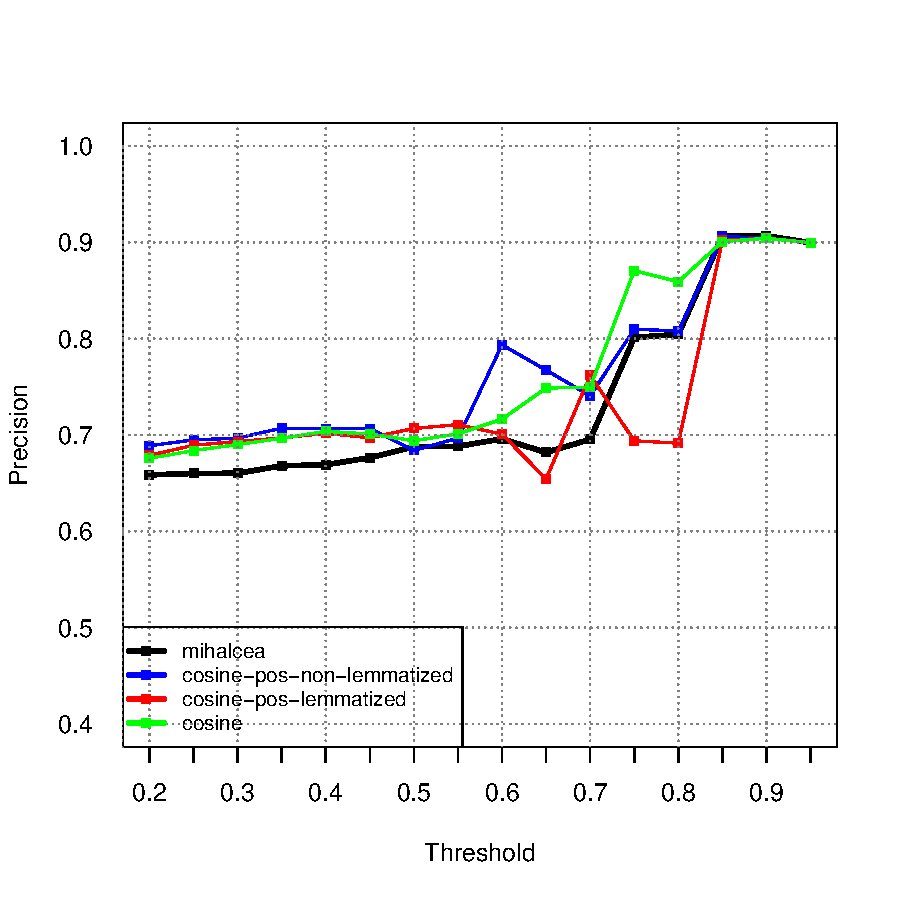
\includegraphics[width=0.5\textwidth]{sweave/sweave-dbscan-minpts-2-eps-0-1-cluster-precision}
\label{fig:dbscan-minpts-2-eps-0-1-precision-cluster}}
\subfloat[Subfigure 2 list of figures text][F1 score - cluster validation strategy]{
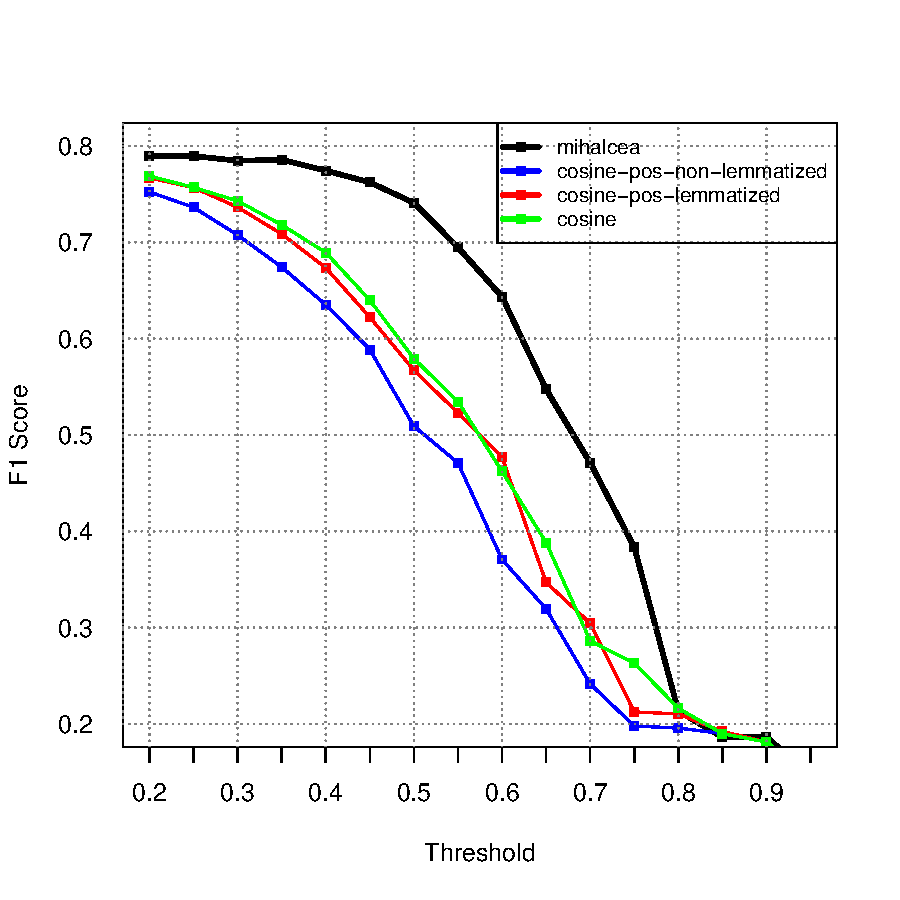
\includegraphics[width=0.5\textwidth]{sweave/sweave-dbscan-minpts-2-eps-0-1-cluster-f1score}
\label{fig:dbscan-minpts-2-eps-0-1-f1score-cluster}}
\qquad
\subfloat[Subfigure 3 list of figures text][Precision - individual validation strategy]{
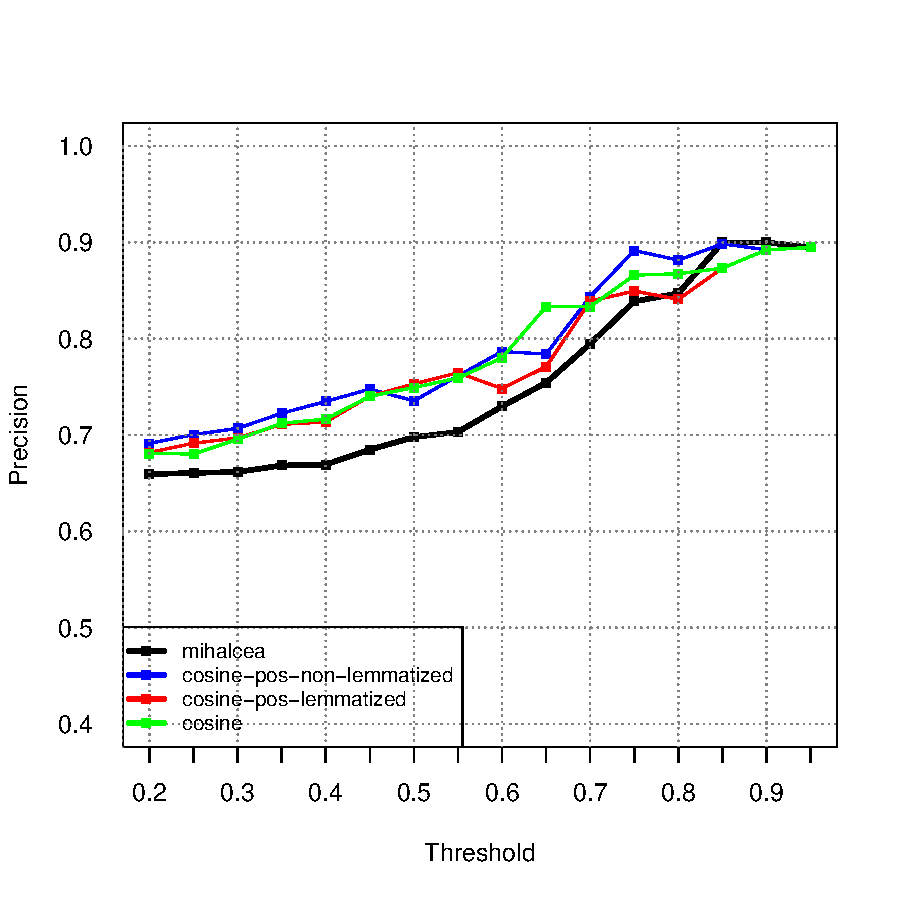
\includegraphics[width=0.5\textwidth]{sweave/sweave-dbscan-minpts-2-eps-0-1-individual-precision}
\label{fig:dbscan-minpts-2-eps-0-1-precision-individual}}
\subfloat[Subfigure 4 list of figures text][F1 score - individual validation strategy]{
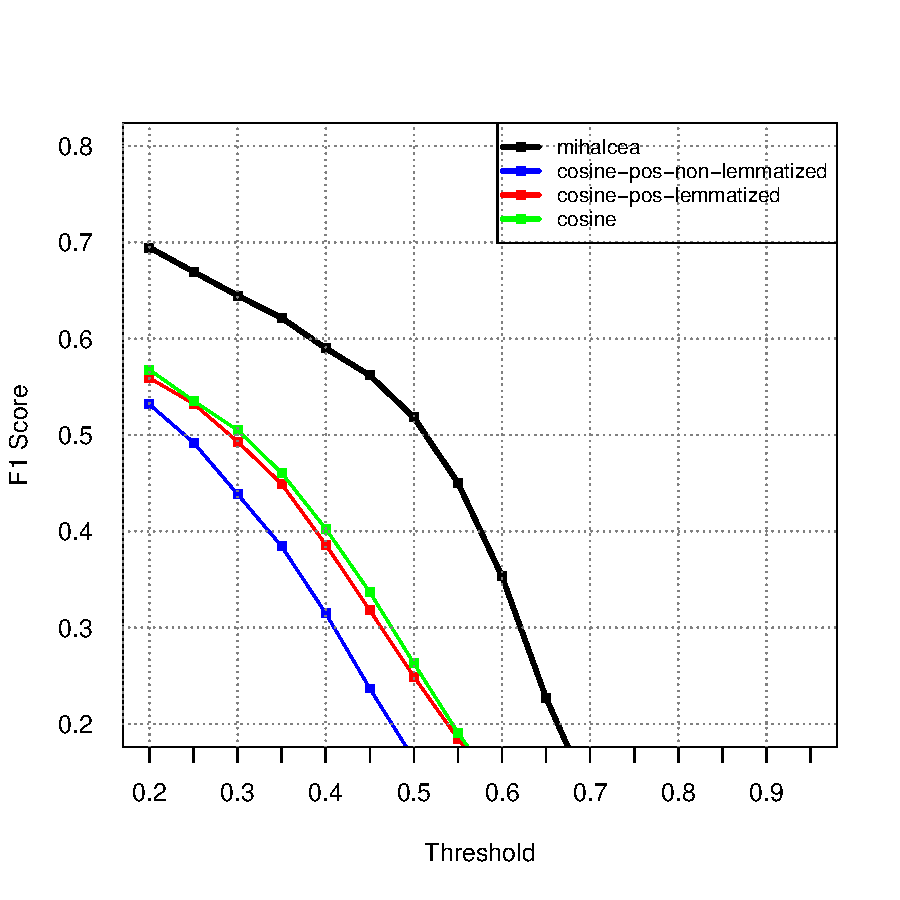
\includegraphics[width=0.5\textwidth]{sweave/sweave-dbscan-minpts-2-eps-0-1-individual-f1score}
\label{fig:dbscan-minpts-2-eps-0-1-f1score-individual}}
\caption{Classifier precision and F1 score for DBSCAN with minPts=2 and epsilon=0.1 using both the cluster and the individual review pair validation strategies}    
\label{dbscan-minpts-2-eps-0-1}
\end{center}
\end{figure}

\begin{figure}[ht]
\begin{center}
\subfloat[Subfigure 1 list of figures text][Precision - cluster validation strategy]{
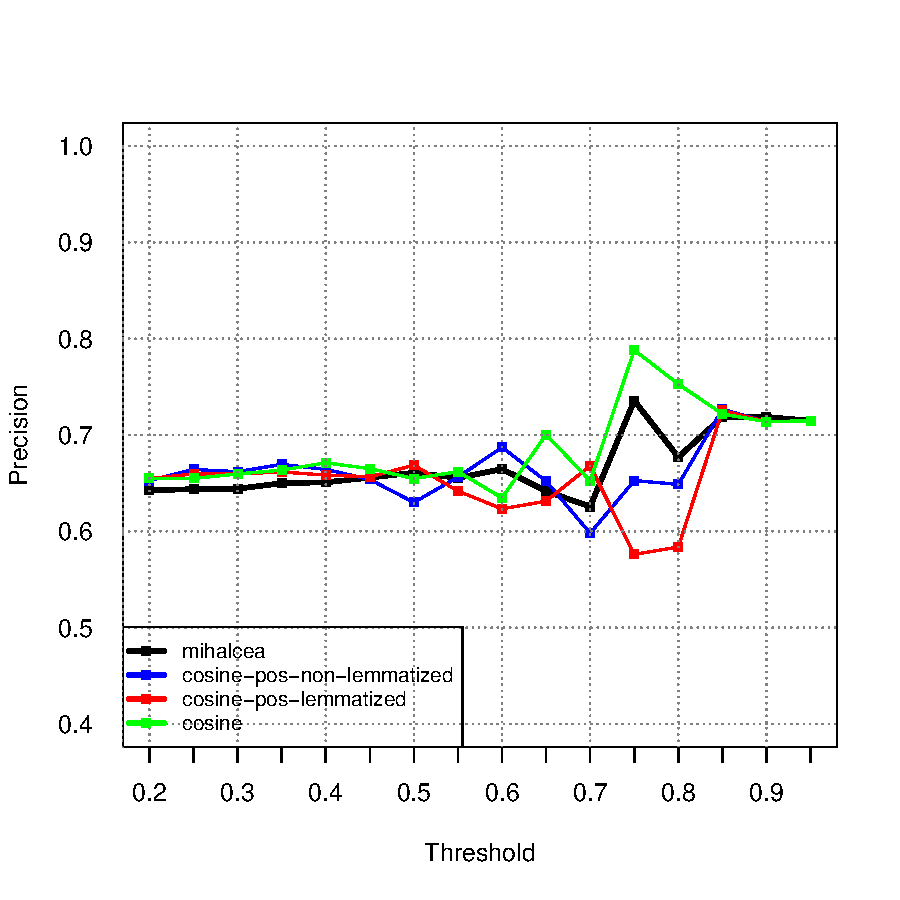
\includegraphics[width=0.5\textwidth]{sweave/sweave-dbscan-minpts-2-eps-0-08-cluster-precision}
\label{fig:subfig1}}
\subfloat[Subfigure 2 list of figures text][F1 score - cluster validation strategy]{
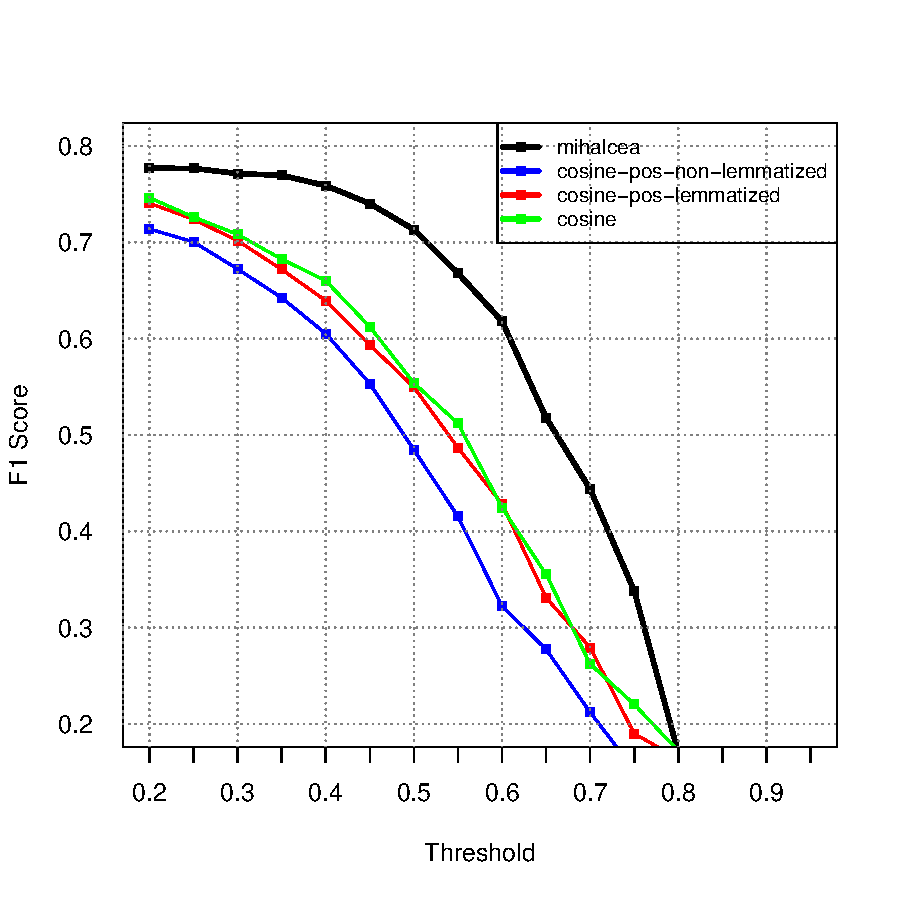
\includegraphics[width=0.5\textwidth]{sweave/sweave-dbscan-minpts-2-eps-0-08-cluster-f1score}
\label{fig:subfig2}}
\qquad
\subfloat[Subfigure 3 list of figures text][Precision - individual validation strategy]{
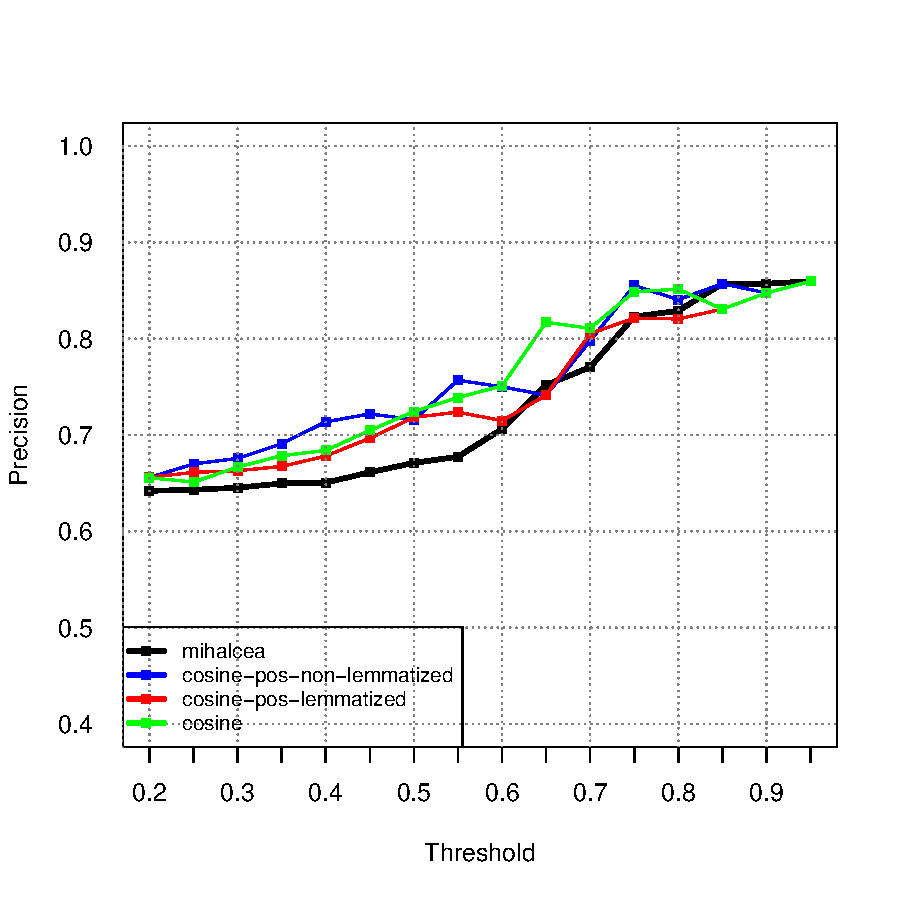
\includegraphics[width=0.5\textwidth]{sweave/sweave-dbscan-minpts-2-eps-0-08-individual-precision}
\label{fig:subfig3}}
\subfloat[Subfigure 4 list of figures text][F1 score - individual validation strategy]{
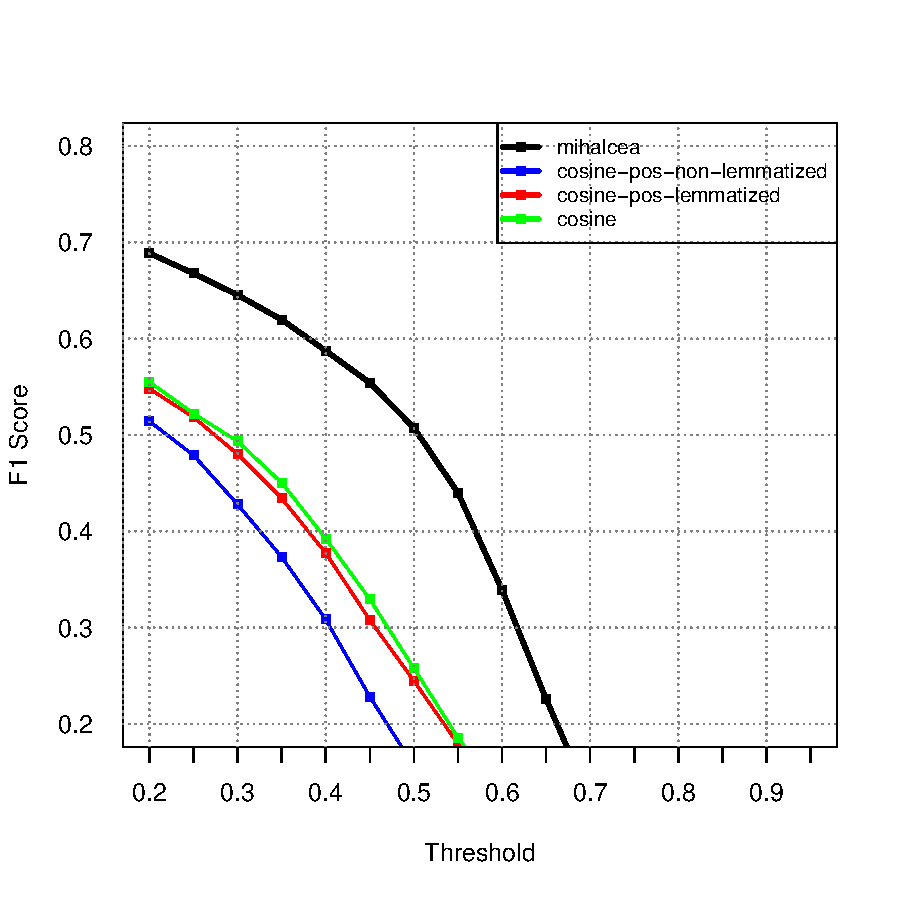
\includegraphics[width=0.5\textwidth]{sweave/sweave-dbscan-minpts-2-eps-0-08-individual-f1score}
\label{fig:subfig4}}
\caption{Classifier precision and F1 score for DBSCAN with minPts=2 and epsilon=0.08 using both the cluster and the individual review pair validation strategies}    
\label{dbscan-minpts-2-eps-0-08}
\end{center}
\end{figure}

\begin{figure}[ht]
\begin{center}
\subfloat[Subfigure 1 list of figures text][Precision - cluster validation strategy]{
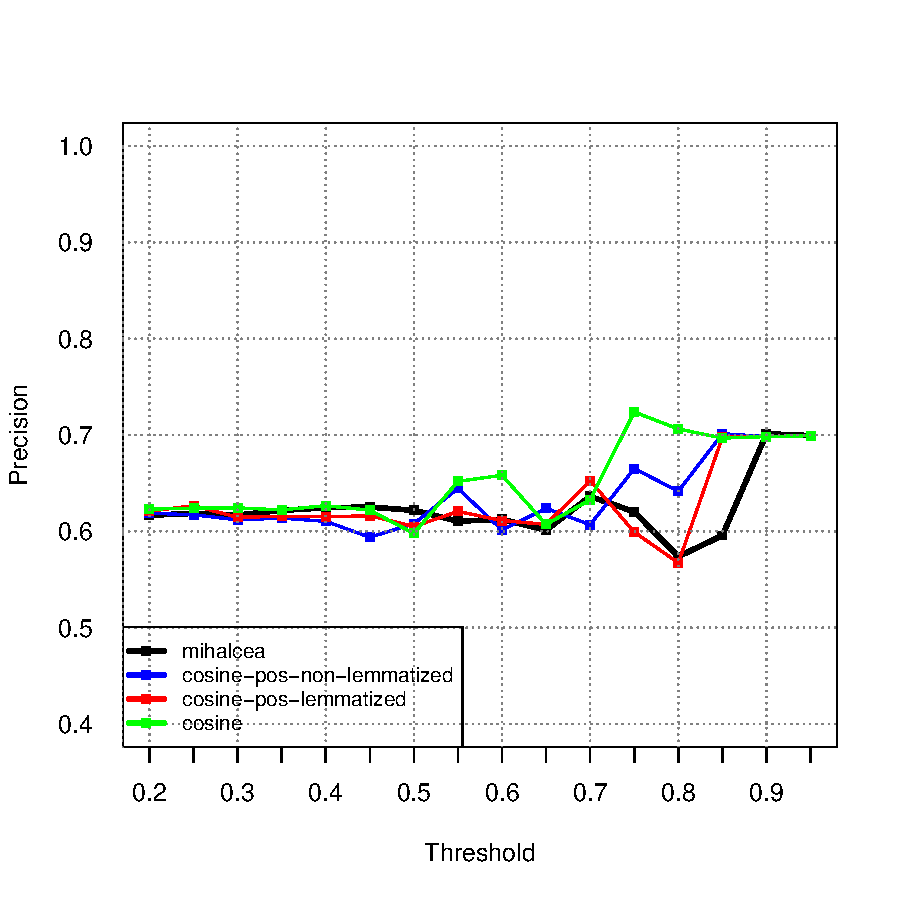
\includegraphics[width=0.5\textwidth]{sweave/sweave-dbscan-minpts-2-eps-0-05-cluster-precision}
\label{fig:subfig1}}
\subfloat[Subfigure 2 list of figures text][F1 score - cluster validation strategy]{
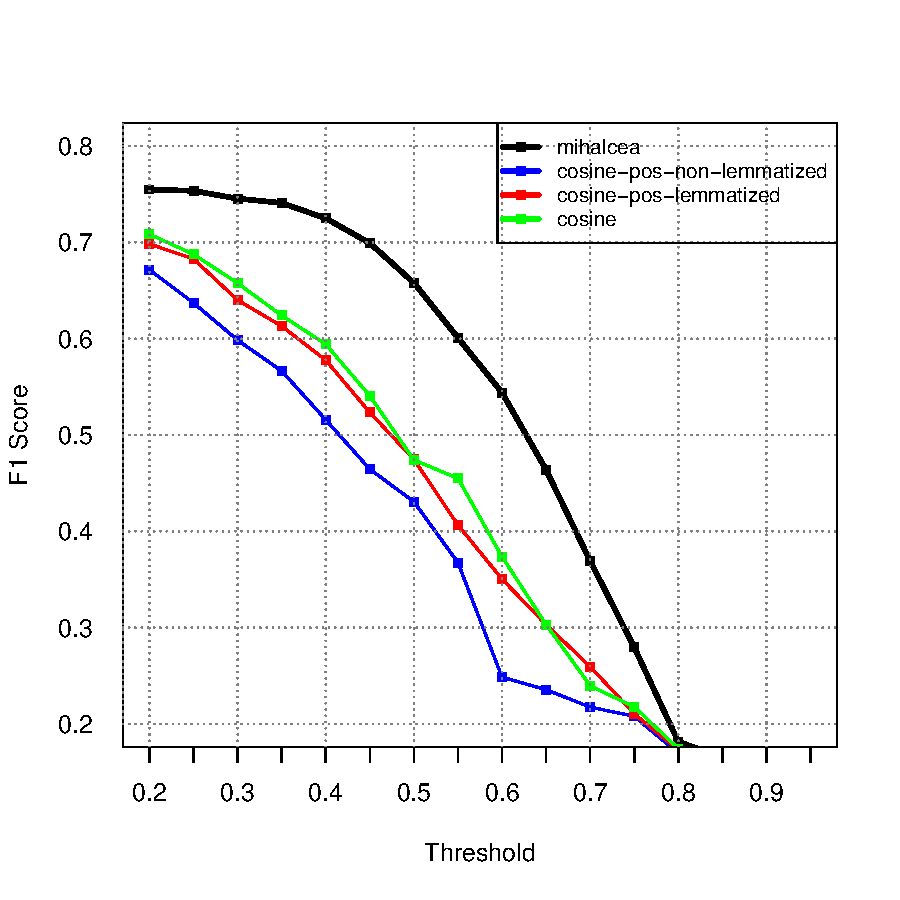
\includegraphics[width=0.5\textwidth]{sweave/sweave-dbscan-minpts-2-eps-0-05-cluster-f1score}
\label{fig:subfig2}}
\qquad
\subfloat[Subfigure 3 list of figures text][Precision - individual validation strategy]{
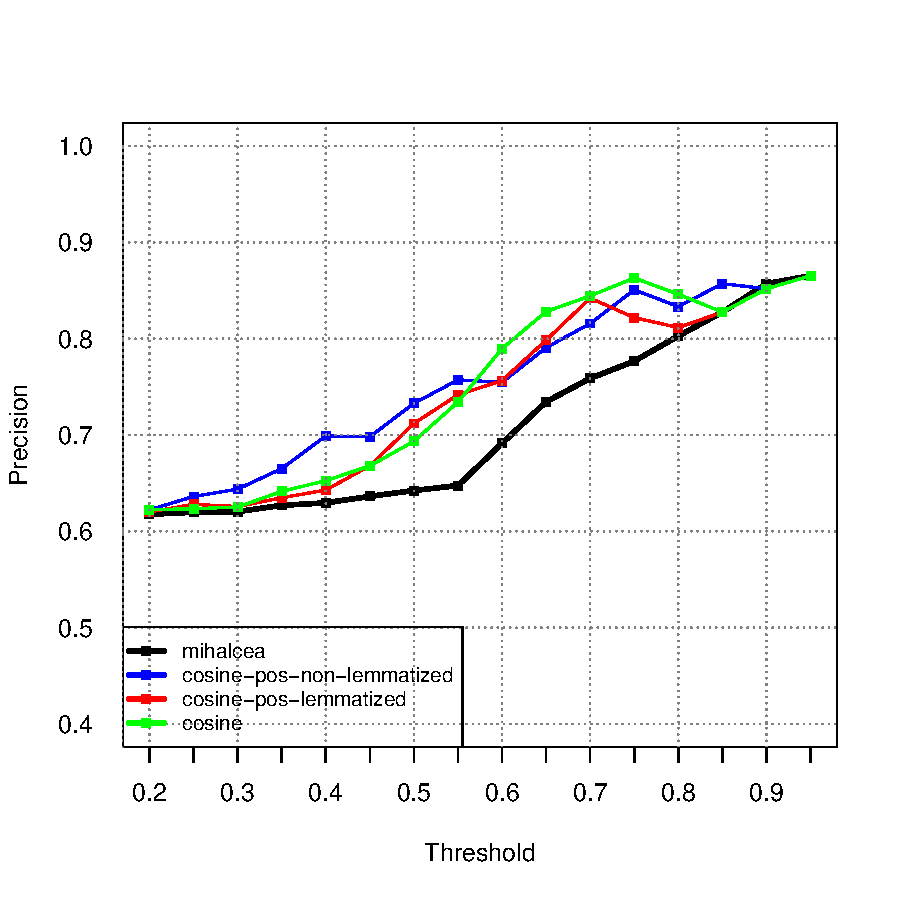
\includegraphics[width=0.5\textwidth]{sweave/sweave-dbscan-minpts-2-eps-0-05-individual-precision}
\label{fig:subfig3}}
\subfloat[Subfigure 4 list of figures text][F1 score - individual validation strategy]{
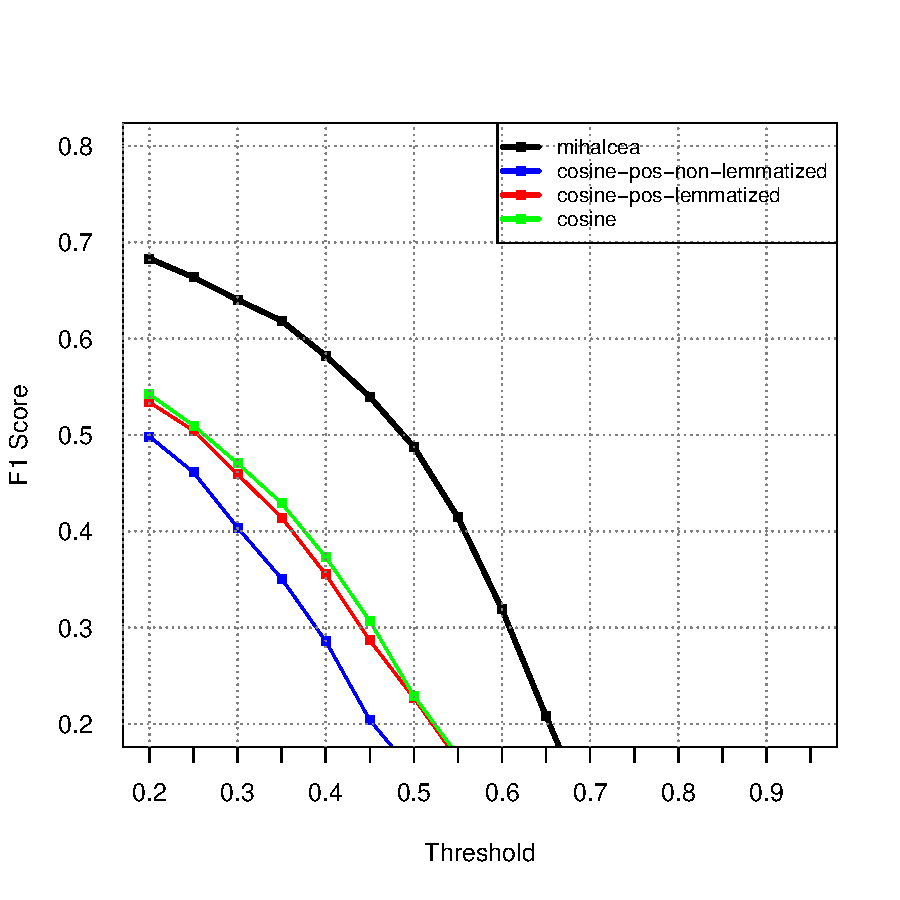
\includegraphics[width=0.5\textwidth]{sweave/sweave-dbscan-minpts-2-eps-0-05-individual-f1score}
\label{fig:subfig4}}
\caption{Classifier precision and F1 score for DBSCAN with minPts=2 and epsilon=0.05 using both the cluster and the individual review pair validation strategies}    
\label{dbscan-minpts-2-eps-0-05}
\end{center}
\end{figure}

\begin{figure}[ht]
\begin{center}
\subfloat[Subfigure 1 list of figures text][Precision - cluster validation strategy]{
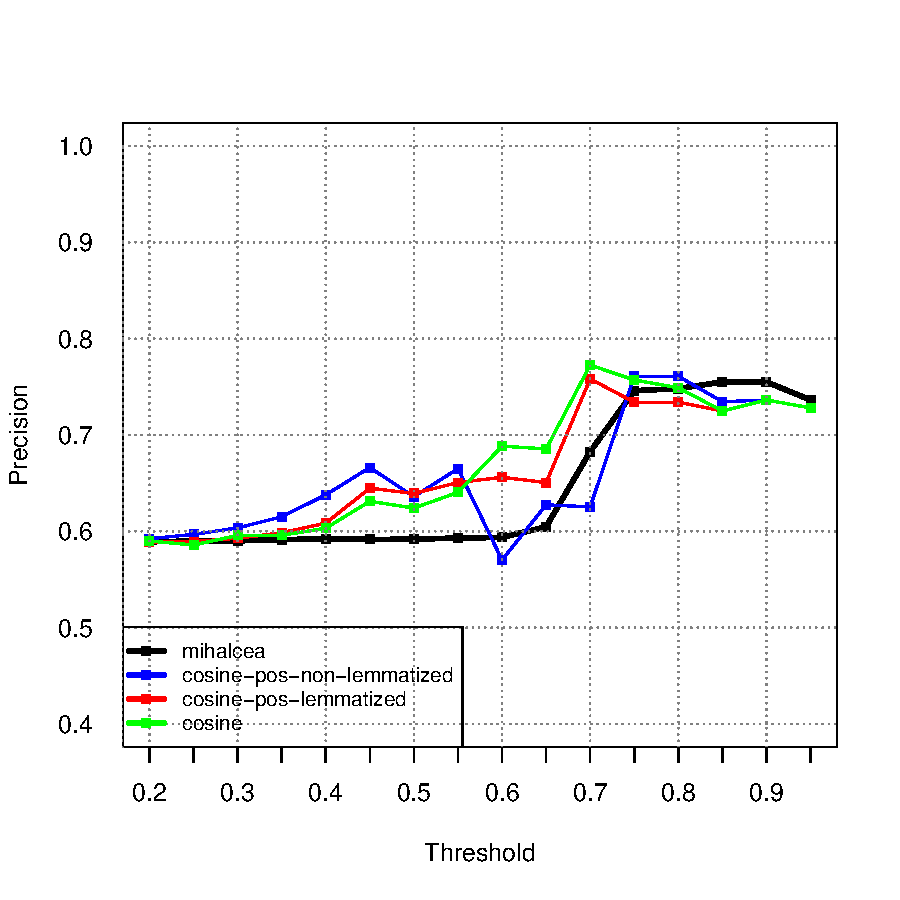
\includegraphics[width=0.5\textwidth]{sweave/sweave-optics-minpts-2-cluster-precision}
\label{fig:subfig1}}
\subfloat[Subfigure 2 list of figures text][F1 score - cluster validation strategy]{
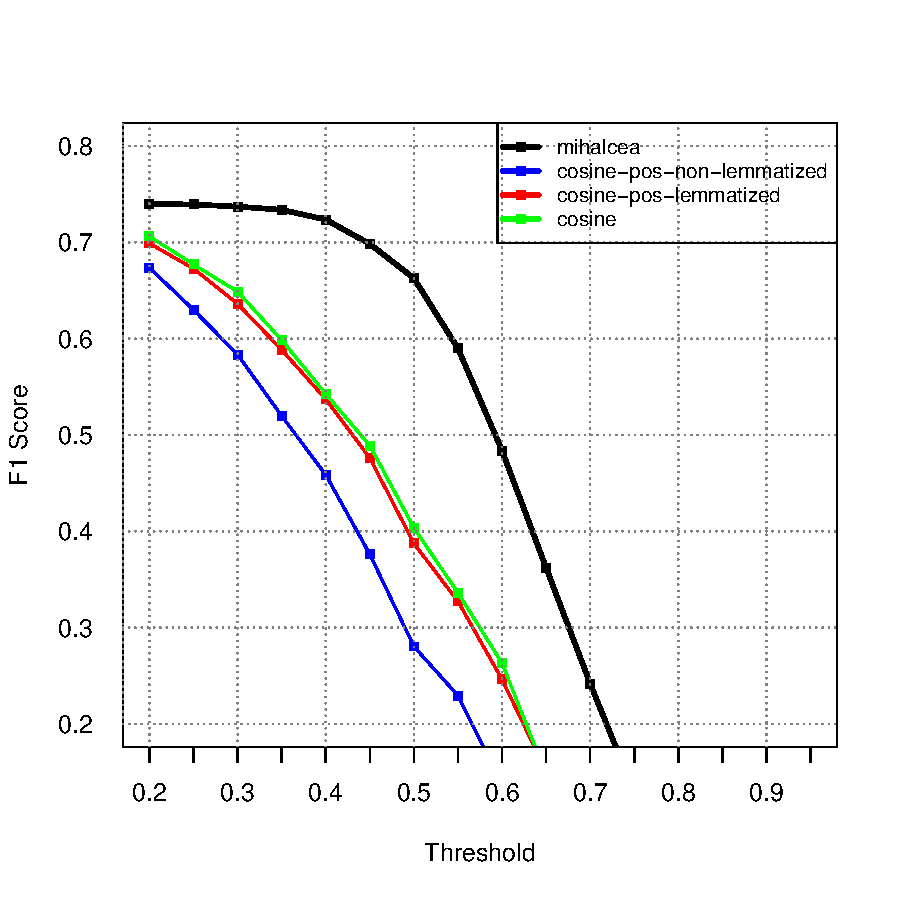
\includegraphics[width=0.5\textwidth]{sweave/sweave-optics-minpts-2-cluster-f1score}
\label{fig:subfig2}}
\qquad
\subfloat[Subfigure 3 list of figures text][Precision - individual validation strategy]{
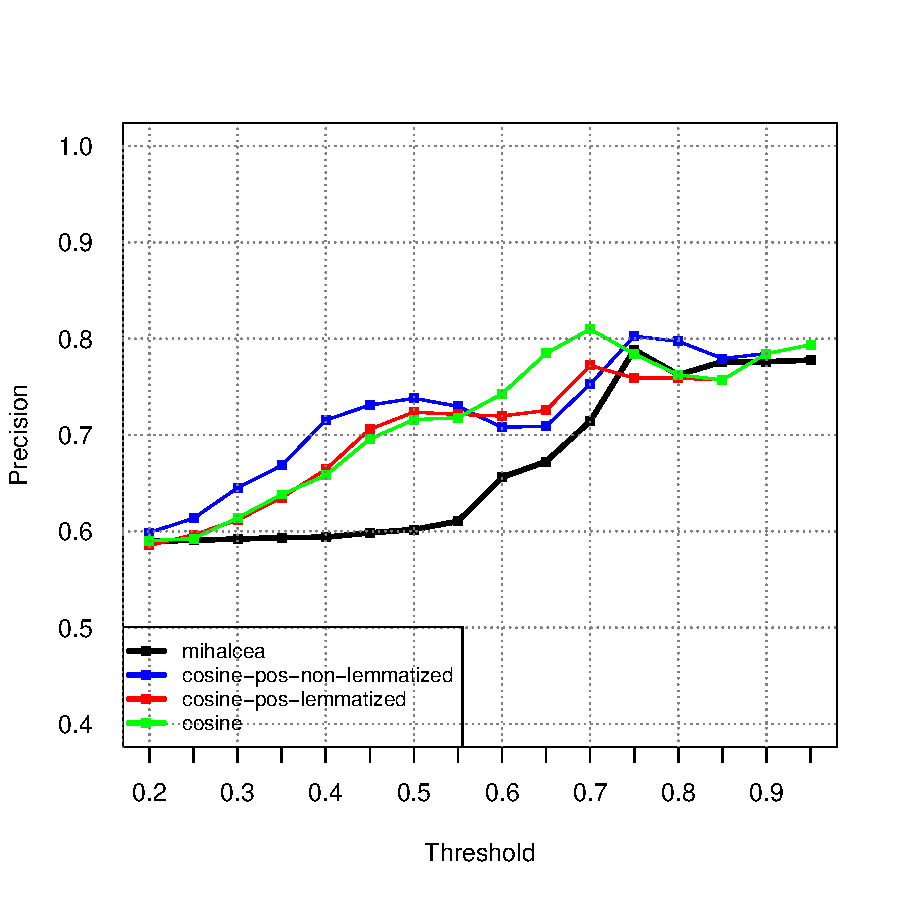
\includegraphics[width=0.5\textwidth]{sweave/sweave-optics-minpts-2-individual-precision}
\label{fig:subfig3}}
\subfloat[Subfigure 4 list of figures text][F1 score - individual validation strategy]{
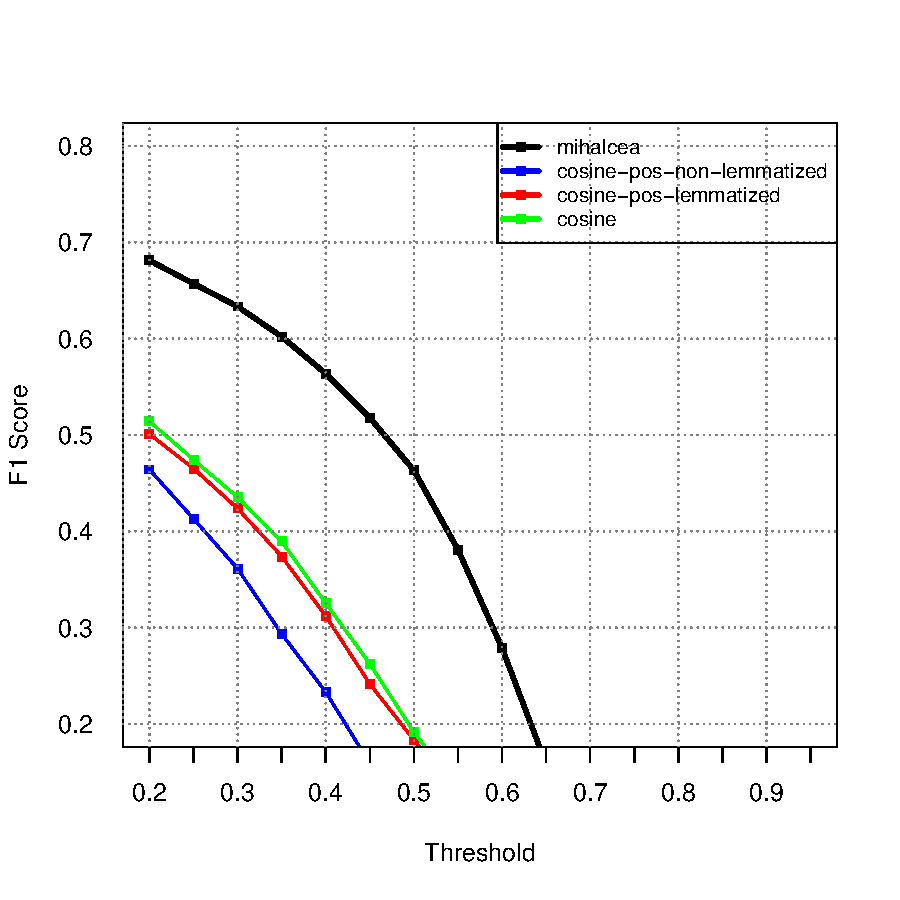
\includegraphics[width=0.5\textwidth]{sweave/sweave-optics-minpts-2-individual-f1score}
\label{fig:subfig4}}
\caption{Classifier precision and F1 score for OPTICS with minPts=2 using both the cluster and the individual review pair validation strategies}    
\label{optics-minpts-2}
\end{center}
\end{figure}

\clearpage
The exact numbers behind the previous plots for both DBSCAN and OPTICS clustering algorithms are shown in Tables \ref{tab:dbscan-minpts-2-eps-0-1-cluster} - \ref{tab:optics-minpts-2-individual}. 

Table \ref{tab:legend} describes the short names used for the columns in each of the results tables. 

\begin{table}[h]
\begin{center}
    \begin{tabular}{ | p{0.2\textwidth} | p{0.7\textwidth} |}
    \hline
    \textbf{Column} & \textbf{Description} \\ \hline
    T & threshold  \\ \hline
    cos & cosine similarity with all parts-of-speech tags, excluding stopwords \\ \hline
    cpnl & cosine similarity with only non-lemmatized POS - nouns, verbs and adjectives, excluding stopwords \\ \hline
    cpl & cosine similarity with only lemmatized POS - combinations between nouns, verbs and adjectives, excluding stopwords \\ \hline
    mih & mihalcea semantic similarity - combinations between nouns, verbs and adjectives, excluding stopwords\\ \hline
    max & \textit{maxsim} - maximum value among of all the previous measures \\ \hline
    P/R/A/F & precision/recall/accuracy/F1-score \\ \hline
    \end{tabular}
\caption{Description of the column names used in the results tables}
\label{tab:legend}
\end{center}
\end{table}
\begin{center}
% latex table generated in R 3.0.2 by xtable 1.7-3 package
% Tue Jul 01 18:39:50 2014
\begin{table}[!h]
\centering
\begin{tabular}{|l|l|l|l|l|l|l|l|l|l|l|}
  \hline
T & cos & cos & cos & cos & cpnl & cpnl & cpnl & cpnl & cpl & cpl \\ 
  \hline
T & P & R & A & F & P & R & A & F & P & R \\ 
   \hline
0.5 & 0.70 & 0.50 & 0.53 & 0.58 & 0.68 & 0.41 & 0.49 & 0.51 & 0.71 & 0.48 \\ 
  0.6 & 0.72 & 0.34 & 0.48 & 0.46 & 0.79 & 0.24 & 0.46 & 0.37 & 0.70 & 0.36 \\ 
  0.7 & 0.75 & 0.18 & 0.42 & 0.29 & 0.74 & 0.14 & 0.40 & 0.24 & 0.76 & 0.19 \\ 
  0.8 & 0.86 & 0.12 & 0.41 & 0.22 & 0.81 & 0.11 & 0.40 & 0.20 & 0.69 & 0.12 \\ 
  0.9 & 0.90 & 0.10 & 0.40 & 0.18 & 0.90 & 0.10 & 0.40 & 0.18 & 0.90 & 0.10 \\ 
   \hline
\end{tabular}
\end{table}
% latex table generated in R 3.0.2 by xtable 1.7-3 package
% Tue Jul 01 18:39:50 2014
\begin{table}[!h]
\centering
\begin{tabular}{|l|l|l|l|l|l|l|l|l|l|l|}
  \hline
T & cpl & cpl & mih & mih & mih & mih & max & max & max & max \\ 
  \hline
T & A & F & P & R & A & F & P & R & A & F \\ 
   \hline
0.5 & 0.53 & 0.57 & 0.69 & 0.80 & 0.63 & 0.74 & 0.69 & 0.81 & 0.63 & 0.74 \\ 
  0.6 & 0.48 & 0.48 & 0.70 & 0.60 & 0.57 & 0.65 & 0.70 & 0.61 & 0.57 & 0.65 \\ 
  0.7 & 0.43 & 0.30 & 0.70 & 0.36 & 0.47 & 0.47 & 0.70 & 0.36 & 0.48 & 0.47 \\ 
  0.8 & 0.39 & 0.21 & 0.80 & 0.12 & 0.40 & 0.21 & 0.71 & 0.15 & 0.40 & 0.24 \\ 
  0.9 & 0.40 & 0.18 & 0.91 & 0.10 & 0.40 & 0.19 & 0.91 & 0.10 & 0.40 & 0.19 \\ 
   \hline
\end{tabular}
\caption{Classifier results for DBSCAN with minPts=2, epsilon=0.1 using the cluster validation strategy} 
\label{tab:dbscan-minpts-2-eps-0-1-cluster}
\end{table}\end{center}

\begin{center}
% latex table generated in R 3.0.2 by xtable 1.7-3 package
% Tue Jul 01 18:39:50 2014
\begin{table}[!h]
\centering
\begin{tabular}{|l|l|l|l|l|l|l|l|l|l|l|}
  \hline
T & cos & cos & cos & cos & cpnl & cpnl & cpnl & cpnl & cpl & cpl \\ 
  \hline
T & P & R & A & F & P & R & A & F & P & R \\ 
   \hline
0.5 & 0.75 & 0.16 & 0.40 & 0.27 & 0.72 & 0.09 & 0.38 & 0.16 & 0.75 & 0.15 \\ 
  0.6 & 0.78 & 0.07 & 0.37 & 0.13 & 0.79 & 0.04 & 0.36 & 0.07 & 0.75 & 0.07 \\ 
  0.7 & 0.83 & 0.03 & 0.36 & 0.06 & 0.84 & 0.03 & 0.35 & 0.05 & 0.84 & 0.03 \\ 
  0.8 & 0.87 & 0.02 & 0.35 & 0.05 & 0.88 & 0.02 & 0.35 & 0.04 & 0.84 & 0.02 \\ 
  0.9 & 0.89 & 0.02 & 0.35 & 0.04 & 0.89 & 0.02 & 0.35 & 0.04 & 0.89 & 0.02 \\ 
   \hline
\end{tabular}
\end{table}
% latex table generated in R 3.0.2 by xtable 1.7-3 package
% Tue Jul 01 18:39:50 2014
\begin{table}[!h]
\centering
\begin{tabular}{|l|l|l|l|l|l|l|l|l|l|l|}
  \hline
T & cpl & cpl & mih & mih & mih & mih & max & max & max & max \\ 
  \hline
T & A & F & P & R & A & F & P & R & A & F \\ 
   \hline
0.5 & 0.40 & 0.25 & 0.70 & 0.41 & 0.48 & 0.52 & 0.70 & 0.42 & 0.48 & 0.52 \\ 
  0.6 & 0.37 & 0.13 & 0.73 & 0.23 & 0.43 & 0.35 & 0.72 & 0.24 & 0.43 & 0.36 \\ 
  0.7 & 0.36 & 0.06 & 0.79 & 0.07 & 0.37 & 0.12 & 0.79 & 0.07 & 0.37 & 0.13 \\ 
  0.8 & 0.35 & 0.05 & 0.85 & 0.02 & 0.35 & 0.05 & 0.84 & 0.03 & 0.35 & 0.05 \\ 
  0.9 & 0.35 & 0.04 & 0.90 & 0.02 & 0.35 & 0.04 & 0.90 & 0.02 & 0.35 & 0.04 \\ 
   \hline
\end{tabular}
\caption{Classifier results for DBSCAN with minPts=2, epsilon=0.1 using the individual review pair validation strategy} 
\label{tab:dbscan-minpts-2-eps-0-1-individual}
\end{table}\end{center}
\begin{center}
% latex table generated in R 3.0.2 by xtable 1.7-3 package
% Tue Jul 01 18:39:50 2014
\begin{table}[!h]
\centering
\begin{tabular}{|l|l|l|l|l|l|l|l|l|l|l|}
  \hline
T & cos & cos & cos & cos & cpnl & cpnl & cpnl & cpnl & cpl & cpl \\ 
  \hline
T & P & R & A & F & P & R & A & F & P & R \\ 
   \hline
0.5 & 0.62 & 0.30 & 0.48 & 0.41 & 0.63 & 0.18 & 0.46 & 0.28 & 0.64 & 0.29 \\ 
  0.6 & 0.69 & 0.16 & 0.46 & 0.26 & 0.57 & 0.08 & 0.42 & 0.14 & 0.66 & 0.15 \\ 
  0.7 & 0.77 & 0.06 & 0.44 & 0.11 & 0.63 & 0.05 & 0.42 & 0.09 & 0.76 & 0.06 \\ 
  0.8 & 0.75 & 0.05 & 0.43 & 0.09 & 0.76 & 0.05 & 0.43 & 0.09 & 0.73 & 0.05 \\ 
  0.9 & 0.74 & 0.04 & 0.43 & 0.08 & 0.74 & 0.04 & 0.43 & 0.08 & 0.74 & 0.04 \\ 
   \hline
\end{tabular}
\end{table}
% latex table generated in R 3.0.2 by xtable 1.7-3 package
% Tue Jul 01 18:39:50 2014
\begin{table}[!h]
\centering
\begin{tabular}{|l|l|l|l|l|l|l|l|l|l|l|}
  \hline
T & cpl & cpl & mih & mih & mih & mih & max & max & max & max \\ 
  \hline
T & A & F & P & R & A & F & P & R & A & F \\ 
   \hline
0.5 & 0.49 & 0.40 & 0.59 & 0.75 & 0.55 & 0.66 & 0.59 & 0.76 & 0.55 & 0.67 \\ 
  0.6 & 0.45 & 0.25 & 0.59 & 0.41 & 0.49 & 0.49 & 0.59 & 0.43 & 0.49 & 0.50 \\ 
  0.7 & 0.43 & 0.11 & 0.68 & 0.15 & 0.46 & 0.24 & 0.69 & 0.15 & 0.46 & 0.25 \\ 
  0.8 & 0.43 & 0.09 & 0.75 & 0.05 & 0.43 & 0.10 & 0.74 & 0.05 & 0.43 & 0.10 \\ 
  0.9 & 0.43 & 0.08 & 0.76 & 0.05 & 0.43 & 0.09 & 0.76 & 0.05 & 0.43 & 0.09 \\ 
   \hline
\end{tabular}
\caption{Classifier results for OPTICS with minPts=2 using the cluster validation strategy} 
\label{tab:optics-minpts-2-cluster}
\end{table}\end{center}
\begin{center}
% latex table generated in R 3.0.2 by xtable 1.7-3 package
% Tue Jul 01 18:39:50 2014
\begin{table}[!h]
\centering
\begin{tabular}{|l|l|l|l|l|l|l|l|l|l|l|}
  \hline
T & cos & cos & cos & cos & cpnl & cpnl & cpnl & cpnl & cpl & cpl \\ 
  \hline
T & P & R & A & F & P & R & A & F & P & R \\ 
   \hline
0.5 & 0.71 & 0.11 & 0.44 & 0.19 & 0.73 & 0.06 & 0.43 & 0.11 & 0.72 & 0.11 \\ 
  0.6 & 0.74 & 0.04 & 0.42 & 0.08 & 0.71 & 0.02 & 0.42 & 0.05 & 0.72 & 0.04 \\ 
  0.7 & 0.81 & 0.02 & 0.42 & 0.04 & 0.75 & 0.02 & 0.42 & 0.03 & 0.77 & 0.02 \\ 
  0.8 & 0.76 & 0.02 & 0.41 & 0.03 & 0.80 & 0.01 & 0.42 & 0.03 & 0.76 & 0.02 \\ 
  0.9 & 0.78 & 0.01 & 0.41 & 0.03 & 0.78 & 0.01 & 0.41 & 0.03 & 0.78 & 0.01 \\ 
   \hline
\end{tabular}
\end{table}
% latex table generated in R 3.0.2 by xtable 1.7-3 package
% Tue Jul 01 18:39:50 2014
\begin{table}[!h]
\centering
\begin{tabular}{|l|l|l|l|l|l|l|l|l|l|l|}
  \hline
T & cpl & cpl & mih & mih & mih & mih & max & max & max & max \\ 
  \hline
T & A & F & P & R & A & F & P & R & A & F \\ 
   \hline
0.5 & 0.44 & 0.19 & 0.60 & 0.38 & 0.49 & 0.46 & 0.60 & 0.38 & 0.49 & 0.47 \\ 
  0.6 & 0.42 & 0.08 & 0.66 & 0.18 & 0.45 & 0.28 & 0.65 & 0.19 & 0.45 & 0.29 \\ 
  0.7 & 0.42 & 0.04 & 0.71 & 0.03 & 0.42 & 0.07 & 0.72 & 0.04 & 0.42 & 0.07 \\ 
  0.8 & 0.42 & 0.03 & 0.76 & 0.02 & 0.41 & 0.03 & 0.76 & 0.02 & 0.42 & 0.03 \\ 
  0.9 & 0.41 & 0.03 & 0.78 & 0.01 & 0.41 & 0.03 & 0.78 & 0.01 & 0.41 & 0.03 \\ 
   \hline
\end{tabular}
\caption{Classifier results for OPTICS with minPts=2 using the individual review pair validation strategy} 
\label{tab:optics-minpts-2-individual}
\end{table}\end{center}

\clearpage 

\section{Distribution of truthful and deceptive reviews}

The CDF curves plotted in Figures \ref{fig:cdf_trustpilot} - \ref{fig:cdf_ott} reveal several interesting aspects. They show the amount of content similarity for the truthful/fake reviews taken separately as well as the position and bounds for each type and the gaps between the two curves. Regardless of the type of similarity measure used, i.e. vectorial or semantic, the two distributional curves of truthful and fake reviews are clearly separated. For the truthful reviews (blue color), the curve appears towards the left of the plot, while for the fake reviews (red color) it is more towards the right. This means that for any similarity measure applied, for a fixed cumulative percentage value, its corresponding value \textit{$x_t$} for truthful reviews will be lower than the value for deceptive reviews \textit{$x_d$}. 

Figure \ref{fig:cdf_trustpilot_mihalcea} shows the largest discriminative margin between the two curves recorded for the Trustpilot dataset. For example, for a fixed cumulative percentage value of 0.4, 40\% of truthful reviews are bounded by a semantic similarity of only 0.28, compared to the same percentage of fake reviews which are bounded by a similarity value of 0.4. For a cumulative percentage of 0.8, 80\% of truthful reviews are bounded by a semantic similarity value of 0.43, while the fake reviews by 0.52. 

In the case of the Ott dataset, Figure \ref{fig:cdf_ott_mihalcea} shows that for a fixed cumulative percentage value of 0.4, 40\% of truthful reviews are bounded by a semantic similarity of only 0.22, compared to the same percentage of fake reviews which are bounded by a similarity value of 0.32. For a cumulative percentage of 0.8, 80\% of truthful reviews are bounded by a semantic similarity value of 0.38, while the fake reviews by 0.44. 

This shows that people writing deceptive reviews tend to have a higher semantic similarity between their reviews than the users writing honest reviews, probably because they are the same person under multiple accounts or know each other and work together. The honest users do not influence each other's writing style so much. The spammers are more likely to do that.

It appears that in both datasets, this gap is not so prominent for the cosine-based measures and this shows that by using the vectorial measures, it becomes harder to differentiate between the truthful and the deceptive reviews. For the Trustpilot dataset, Figure \ref{fig:cdf_trustpilot_cosine} shows that 40\% of truthful reviews are bounded by a cosine similarity value of 0.08, compared to only 0.1 for fake reviews. The difference of 0.02 is significantly lower then the semantic measure which showed a larger gap of 0.12. 

\begin{figure}[ht]
\begin{center}
\subfloat[Subfigure 1 list of figures text][Mihalcea]{
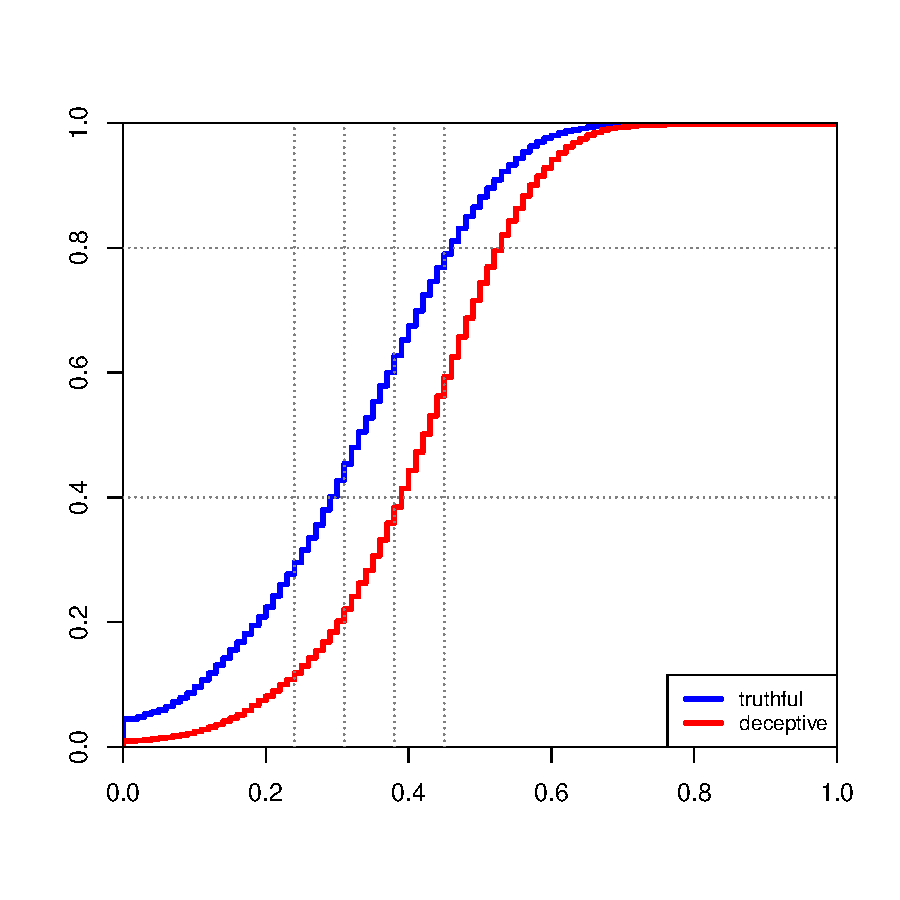
\includegraphics[width=0.5\textwidth]{sweave/sweave-trustpilotmihalceacdf}
\label{fig:cdf_trustpilot_mihalcea}}
\subfloat[Subfigure 2 list of figures text][Cosine]{
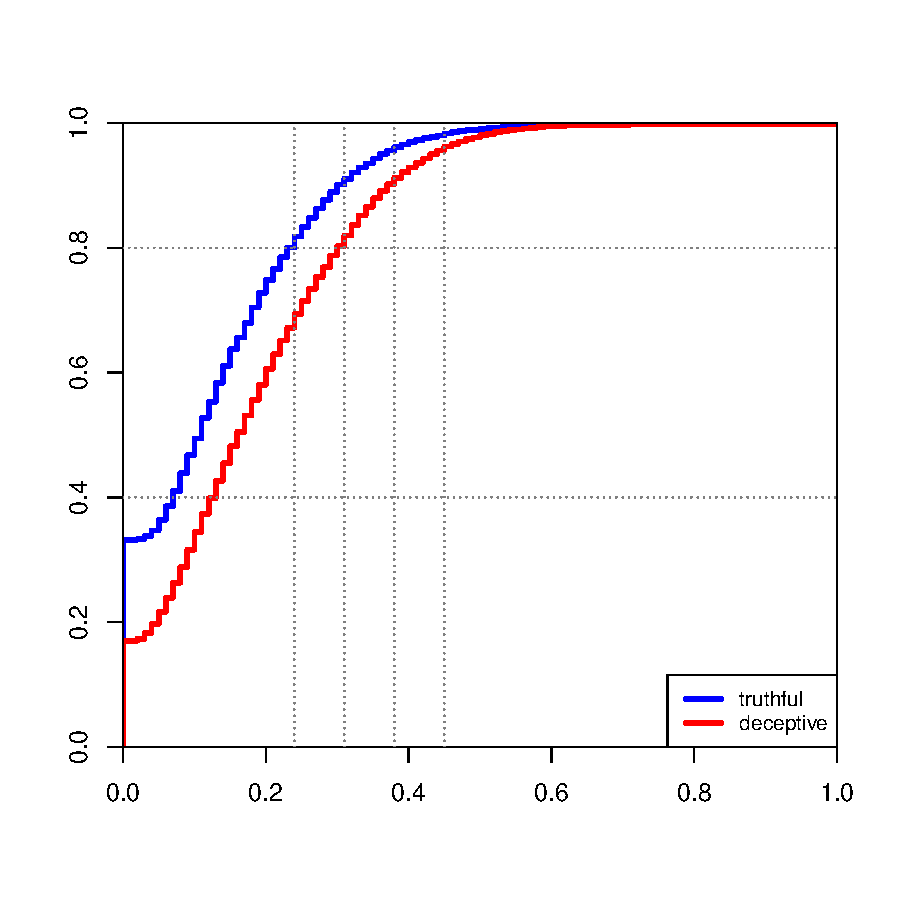
\includegraphics[width=0.5\textwidth]{sweave/sweave-trustpilotcosinecdf}
\label{fig:cdf_trustpilot_cosine}}
\qquad
\subfloat[Subfigure 3 list of figures text][Cosine without lemmatization]{
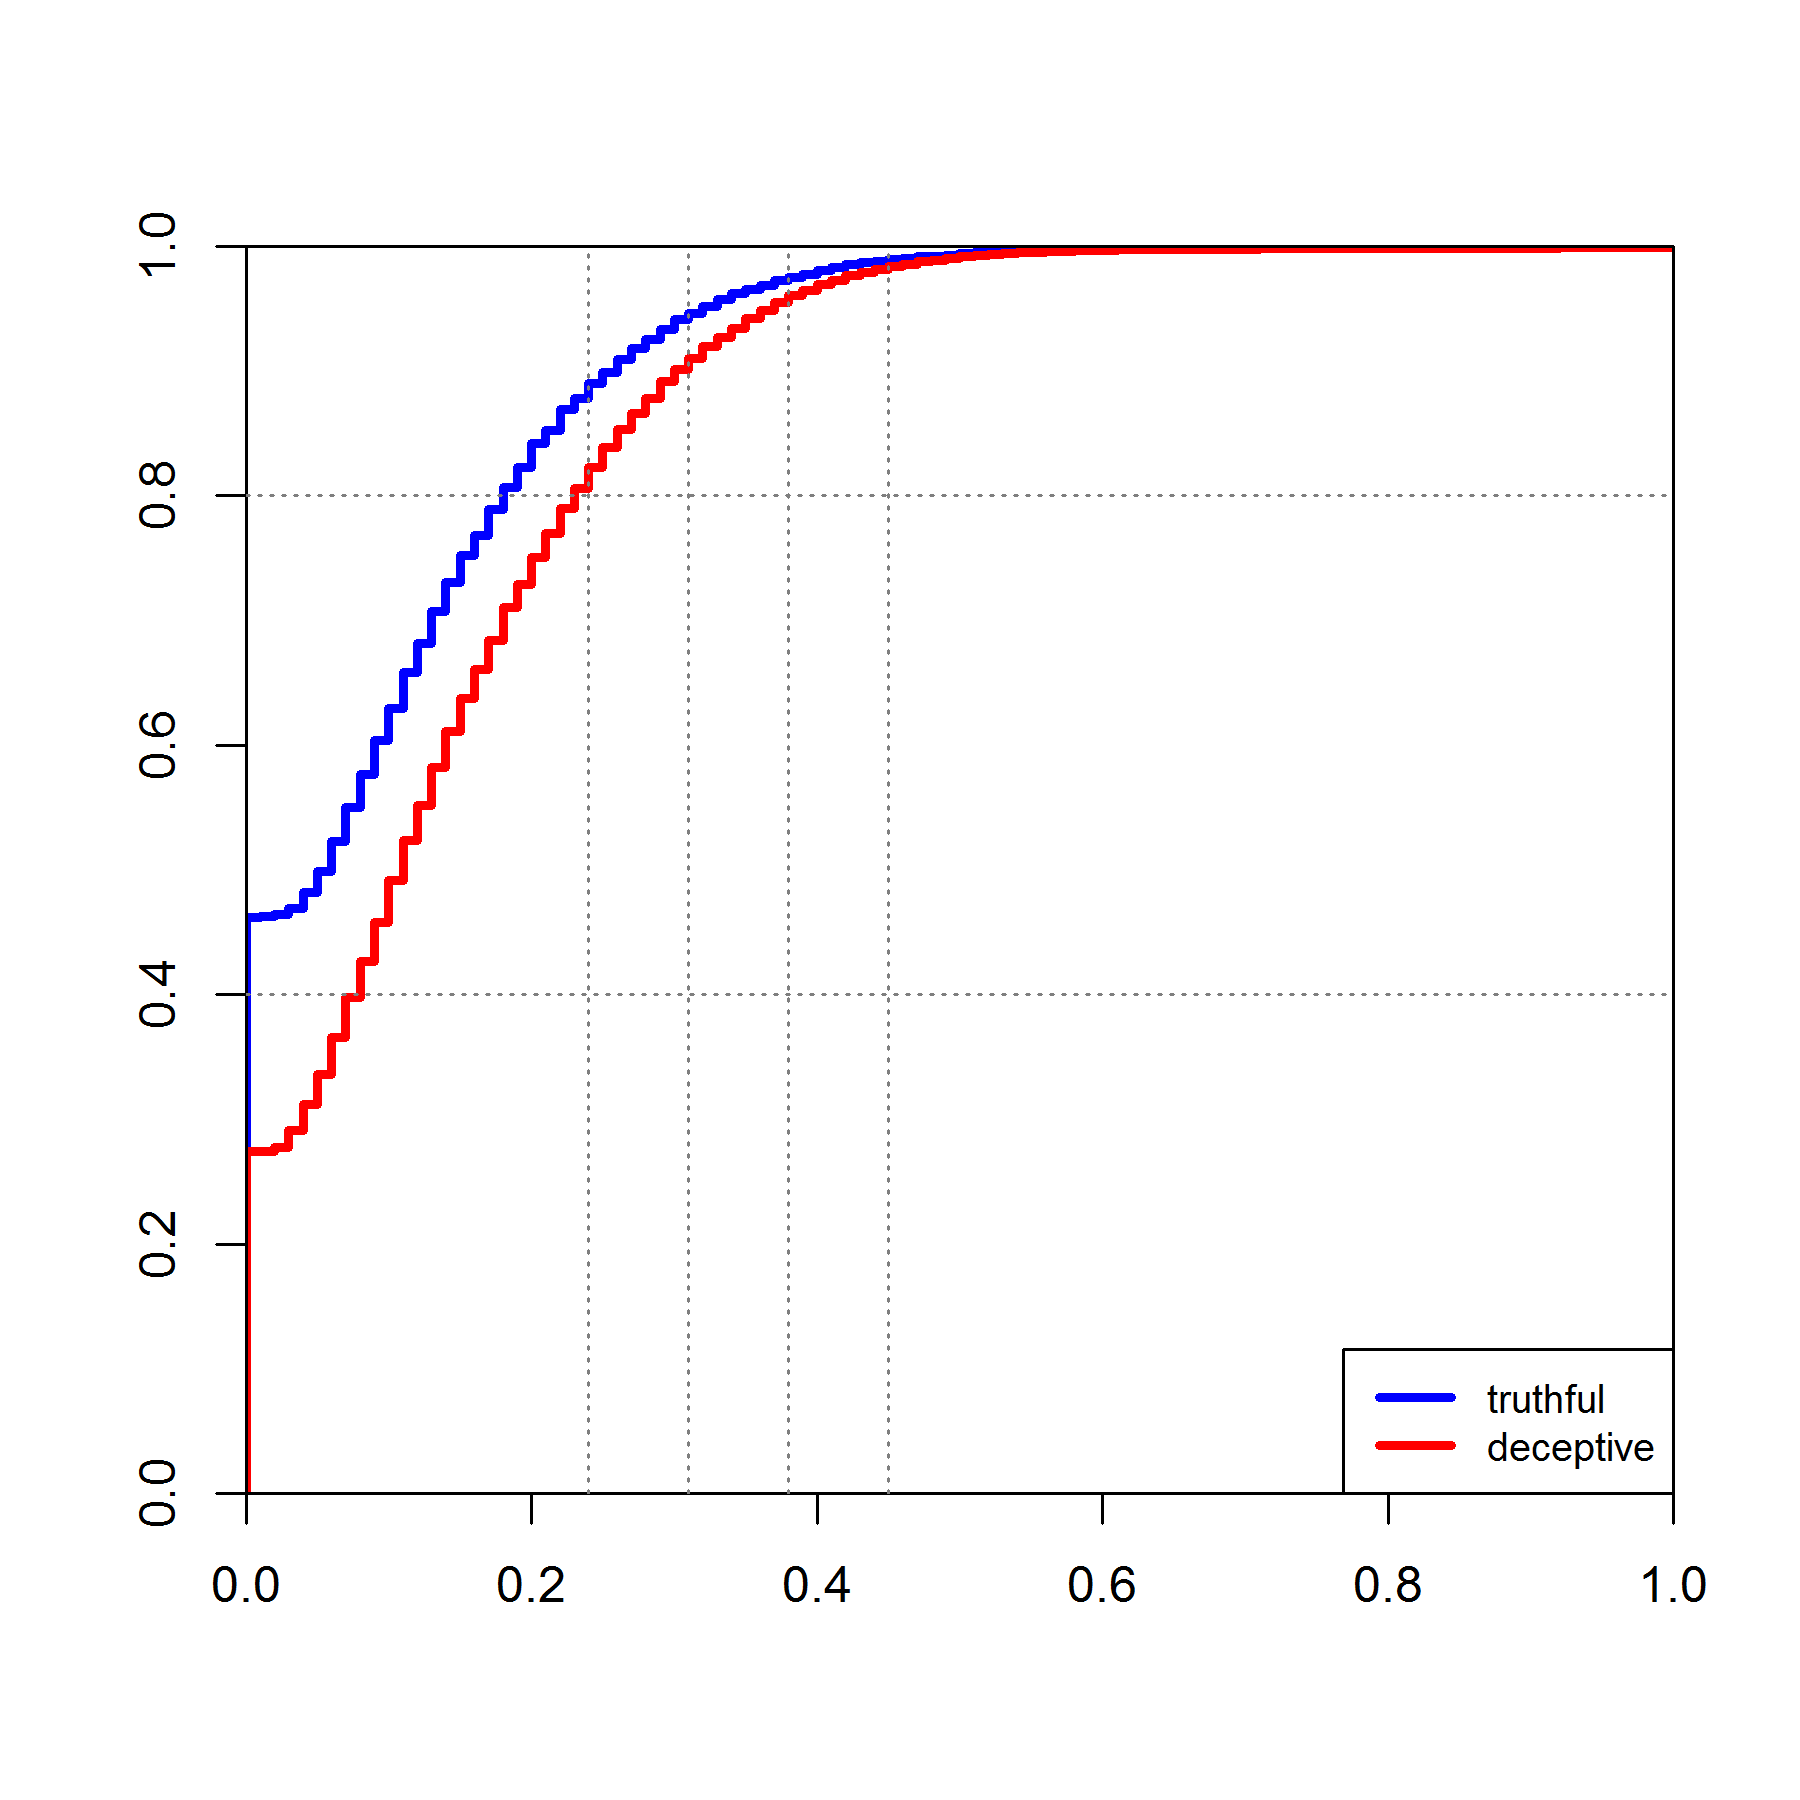
\includegraphics[width=0.5\textwidth]{sweave/sweave-trustpilotcosineposnonlemmatizedcdf}
\label{fig:cdf_trustpilot_cosineposnonlemmatized}}
\subfloat[Subfigure 4 list of figures text][Cosine with lemmatization]{
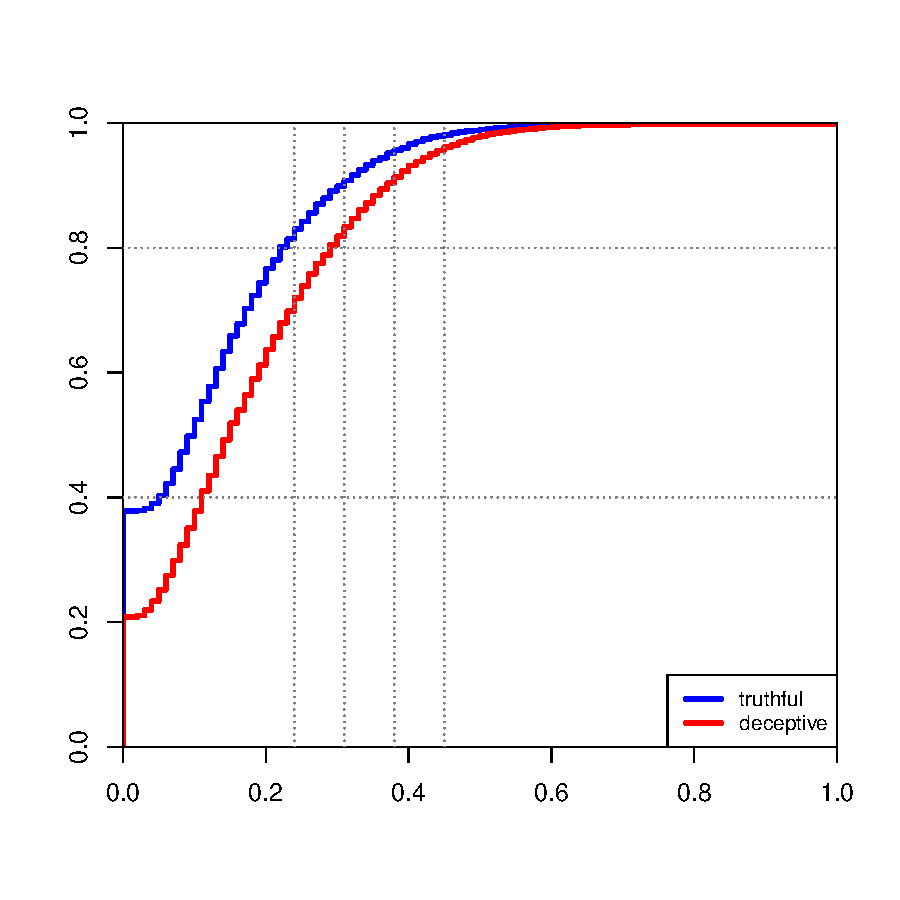
\includegraphics[width=0.5\textwidth]{sweave/sweave-trustpilotcosineposlemmatizedcdf}
\label{fig:cdf_trustpilot_cosineposlemmatized}}
\caption{Trustpilot dataset - cumulative percentage of fake reviews (red color) and truthful reviews (blue color) vs. similarity measures values}    
\label{fig:cdf_trustpilot}
\end{center}
\end{figure}

\begin{figure}[ht]
\begin{center}
\subfloat[Subfigure 1 list of figures text][Mihalcea]{
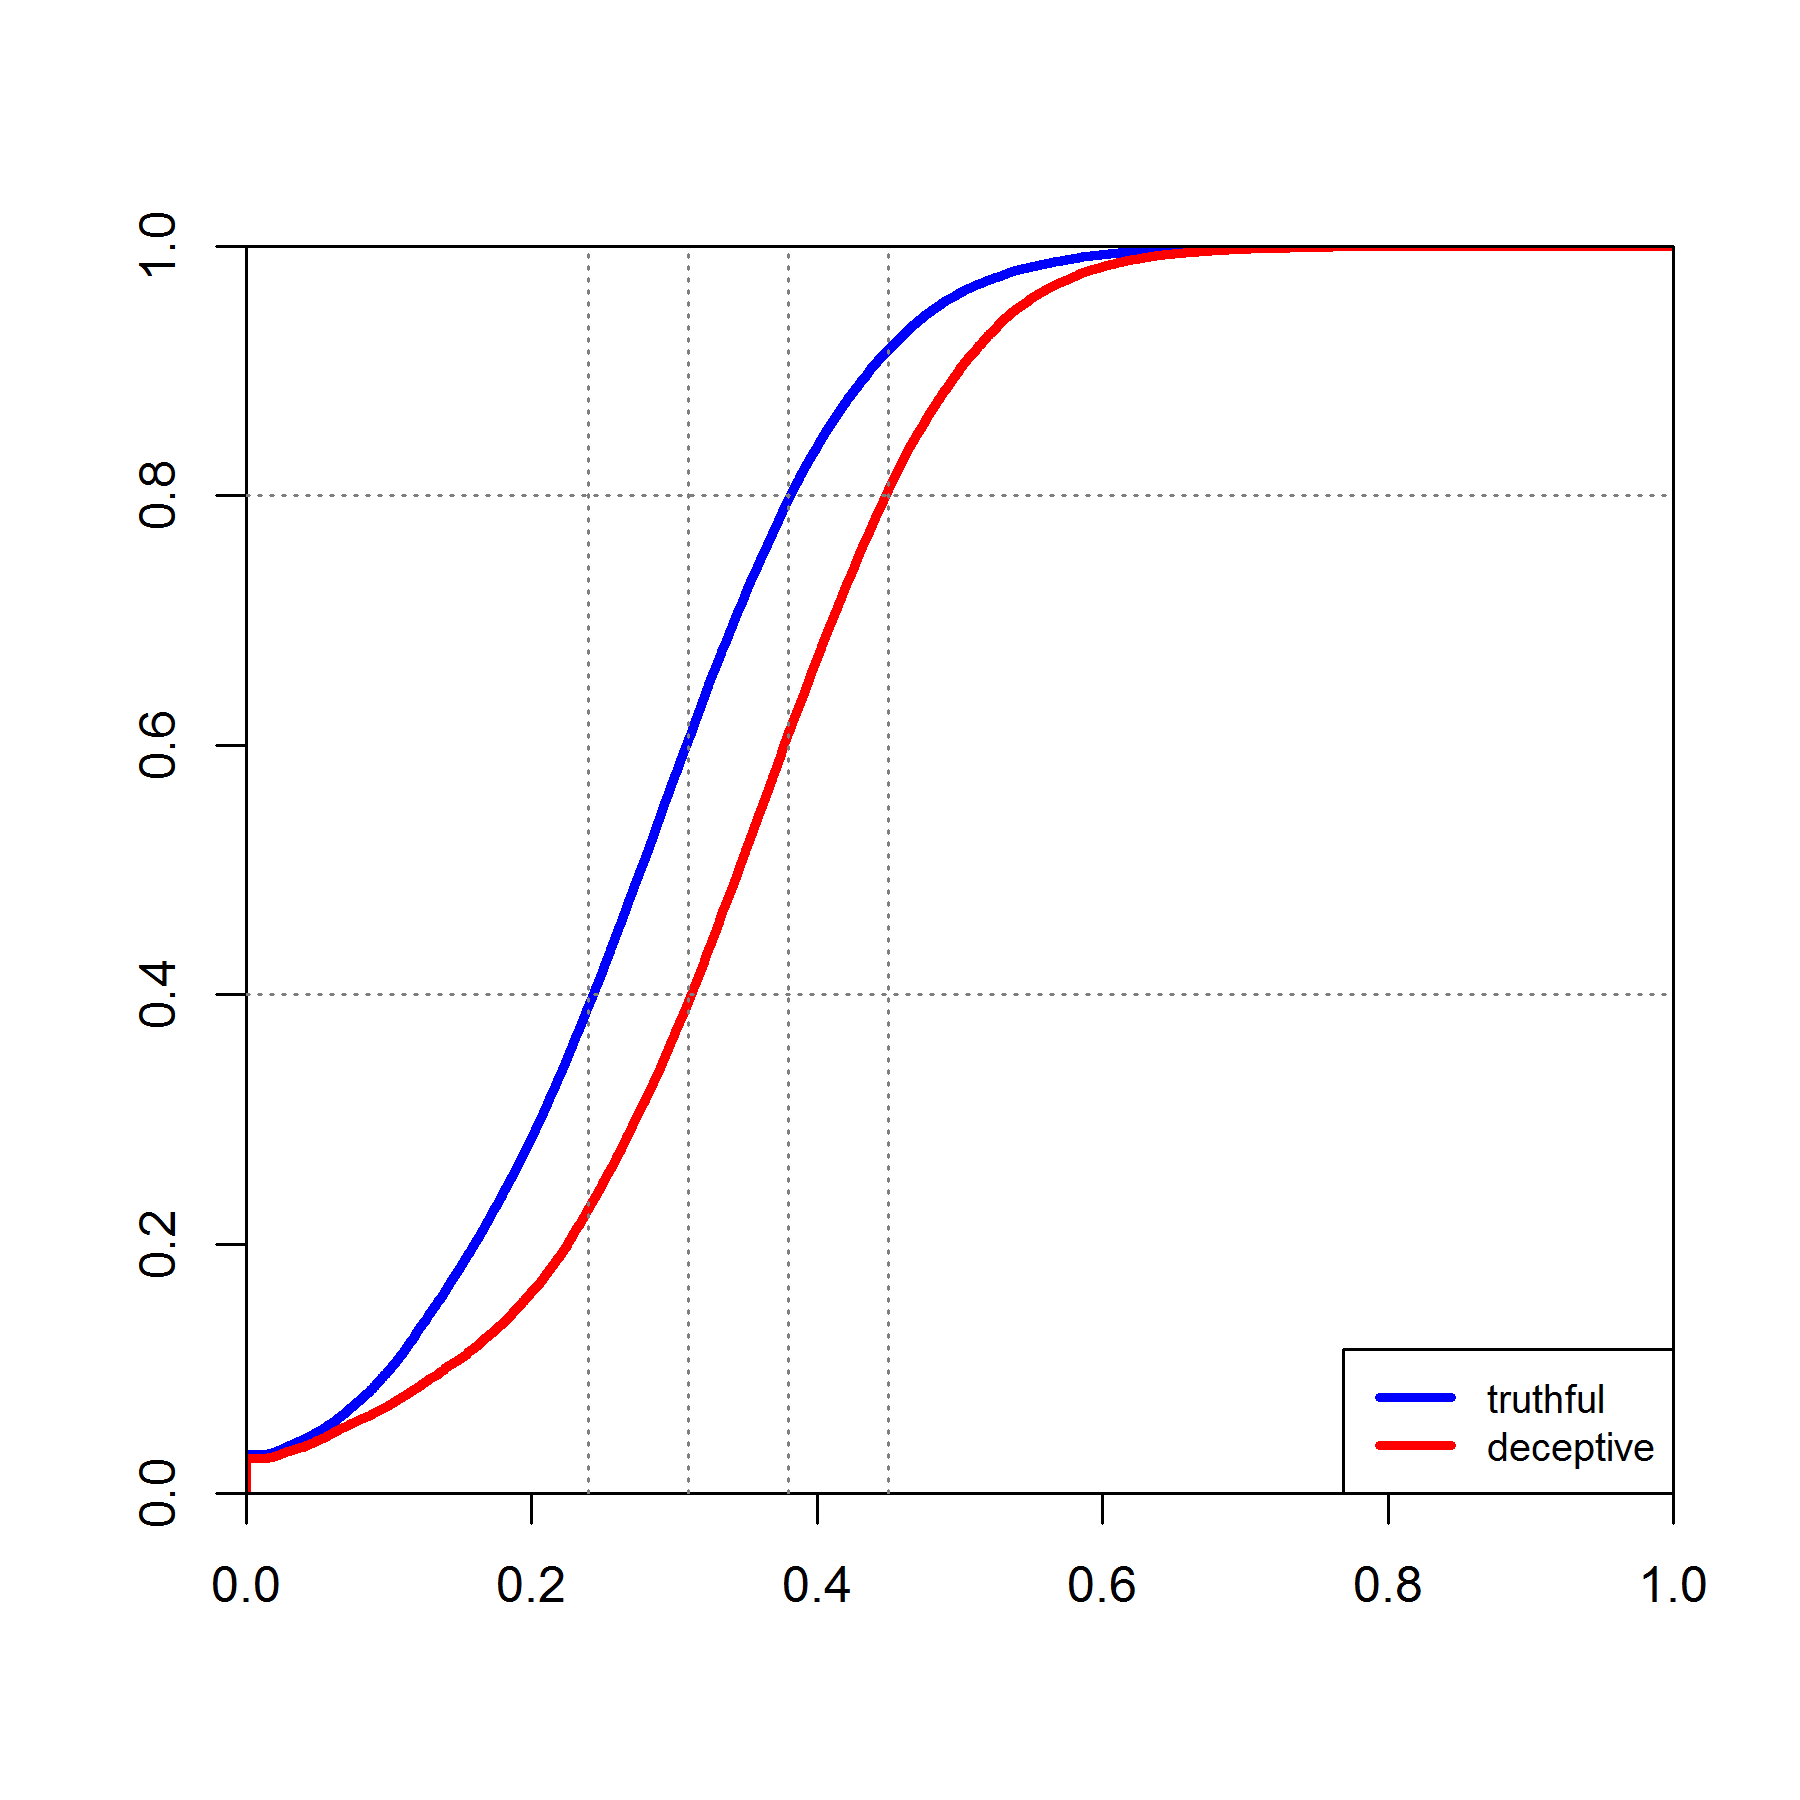
\includegraphics[width=0.5\textwidth]{sweave/sweave-ottmihalcea}
\label{fig:cdf_ott_mihalcea}}
\subfloat[Subfigure 2 list of figures text][Cosine]{
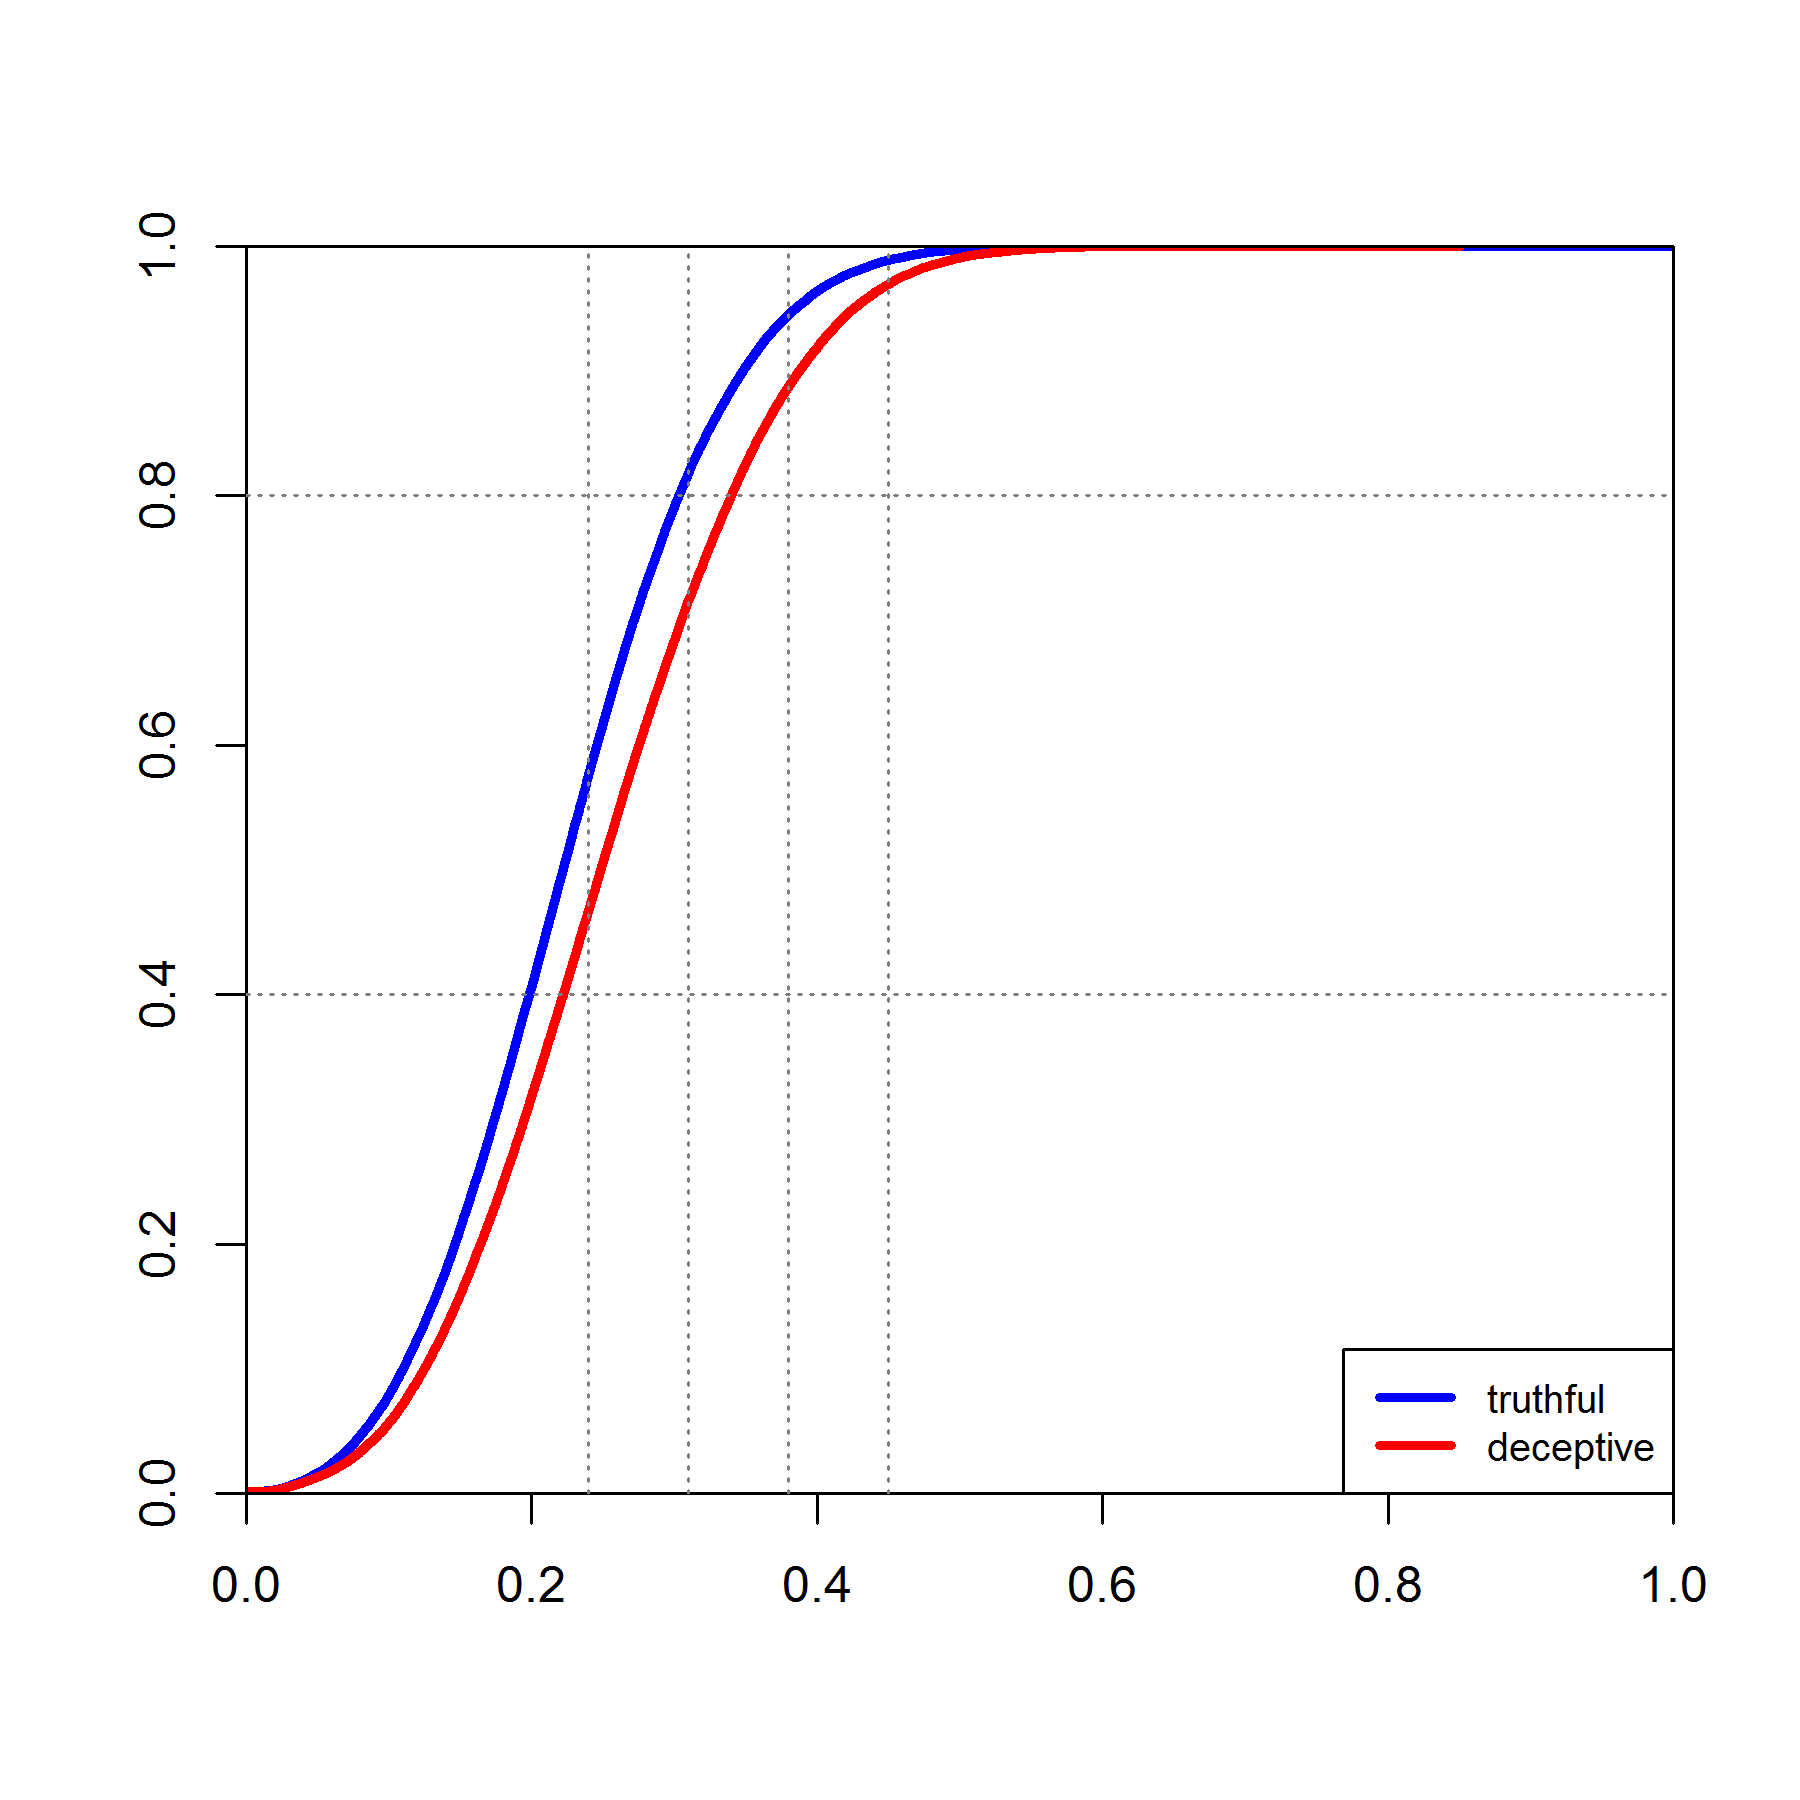
\includegraphics[width=0.5\textwidth]{sweave/sweave-ottcosine}
\label{fig:cdf_ott_cosine}}
\qquad
\subfloat[Subfigure 3 list of figures text][Cosine without lemmatization]{
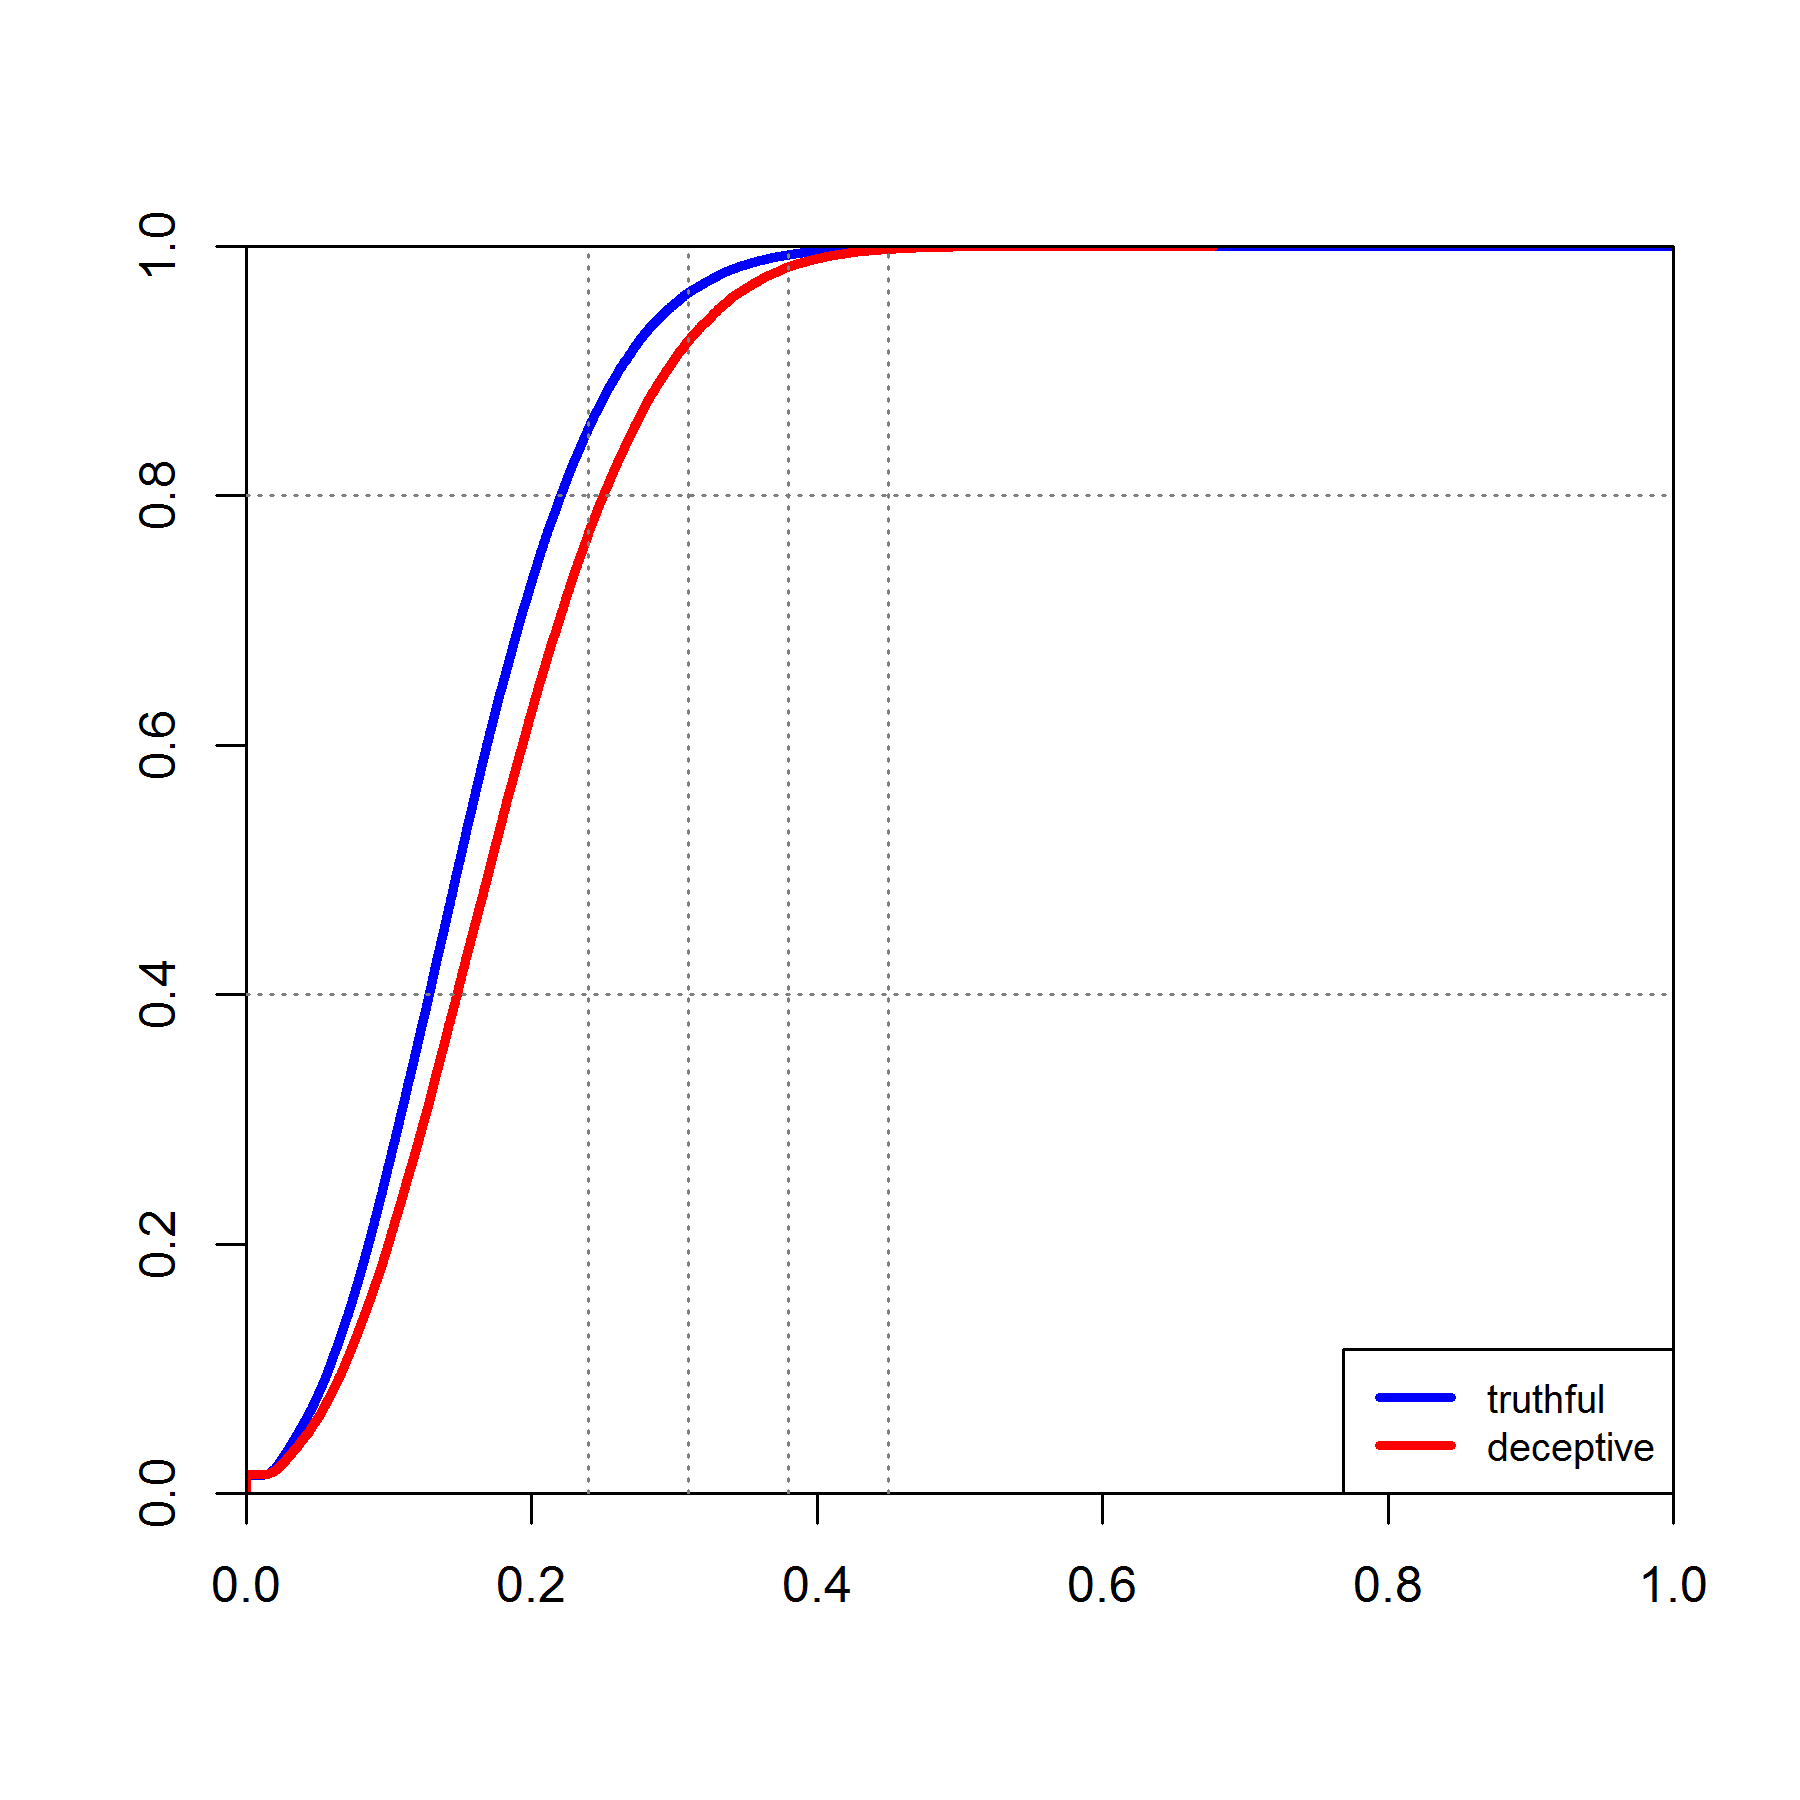
\includegraphics[width=0.5\textwidth]{sweave/sweave-ottcosineposnonlemmatized}
\label{fig:cdf_ott_cosine_without_lemmatization}}
\subfloat[Subfigure 4 list of figures text][Cosine with lemmatization]{
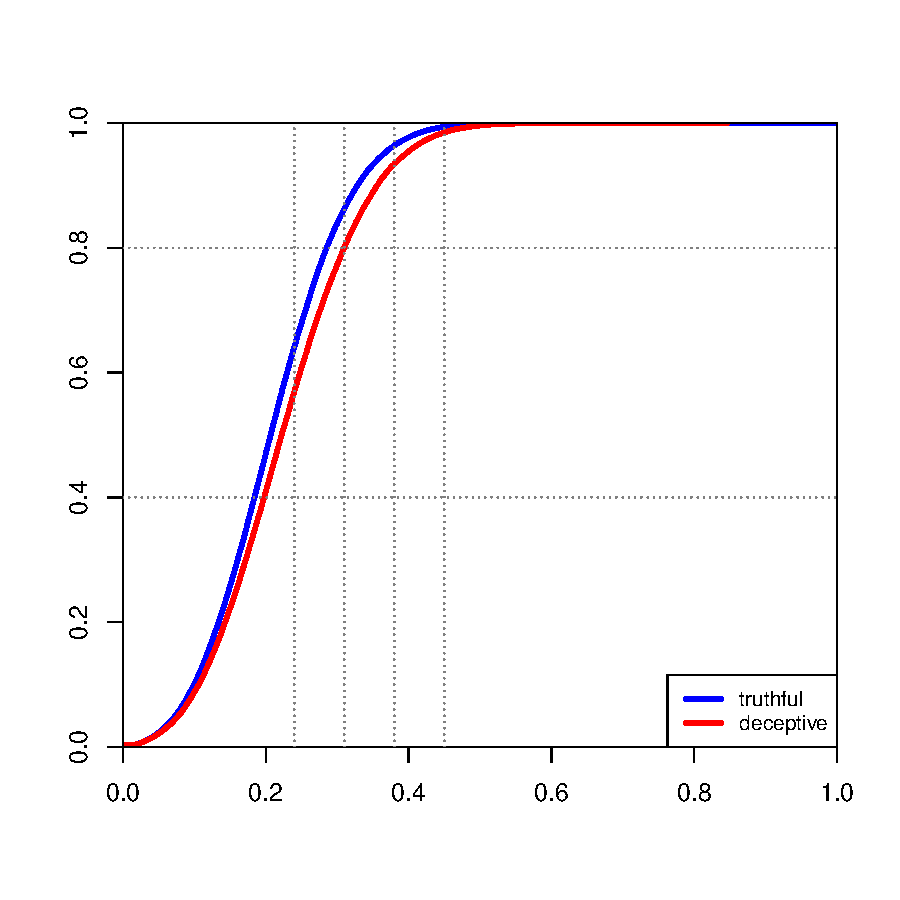
\includegraphics[width=0.5\textwidth]{sweave/sweave-ottcosineposlemmatized}
\label{fig:cdf_ott_cosine_with_lemmatization}}
\caption{Ott dataset - cumulative percentage of fake reviews (red color) and truthful reviews (blue color) vs. similarity measures values}    
\label{fig:cdf_ott}
\end{center}
\end{figure}

\clearpage 

For the Ott dataset, Figure \ref{fig:cdf_ott_cosine} shows that 80\% of truthful reviews are bounded by a cosine similarity value of 0.32, compared to the 0.34 for fake reviews. The difference is only of 0.2 compared to the semantic similarity measure which showed a gap of 0.6. An even smaller difference can be seen for the cosine with and without lemmatization measures. 

Another interesting aspect observed in the Trustpilot dataset is the steep initial jump of the vectorial measures. The cosine without lemmatization measure in Figure \ref{fig:cdf_trustpilot_cosineposnonlemmatized} shows that almost 25\% of the fake reviews exhibit zero similarity between each other. For the same cumulative percentage, the semantic measure shows a similarity bound of up to 0.32. The cosine and cosine with lemmatization measures in Figures \ref{fig:cdf_trustpilot_cosine} - \ref{fig:cdf_trustpilot_cosineposlemmatized} have a similar distribution with a clear but small gap between the curves with about 50\% of known deceptive reviews having a similarity bound of 0.2. Compared to the semantic measure, only 10\% of the fake reviews have a similarity below this value.

One obvious question is why isn't this gap larger, especially for the semantic similarity measure, regardless of the dataset? 

One possible explanation might be that reviews from the same seller generally talk pretty much about aspects within a very specific context, which is related to the shop's business area of activity. For example, if the shop is an electronics reseller that offers online ordering, home delivery and customer support for sold items, then the review will probably contain aspects related to website, the delivery speed, customer support, service level, screen, battery, price and so on. It is pretty easy for the spammers to mimic the honest reviews in the sense of mentioning the same key aspects in their reviews.

The dataset of \citet{Ott2011} has been created using Amazon Mechanical Turk (AMT), so it is likely the turkers was separate persons and did not know each other. It is a different setup than for the real-life Trustpilot dataset, where the fake reviews are more likely to be written by the same people using multiple accounts on the review platform. \citet{Mukherjee2013a} questioned the validity of using fake reviews obtained through a crowdsourcing service such as AMT to detect real-life deceptive reviews in a commercial website and their results showed a much lower accuracy when testing on real-life Yelp reviews than what \citet{Ott2011} reported in their study. 

To conclude, two other possible explanations for why the gap is not larger might be that first of all, the AMT users were separate persons and second, the crowdsourced data may not be representative of real-life scenarios. 

\clearpage

\section{Aspect-based mining for opinion spam detection}

Figure \ref{fig:lda-words-all-hist} shows the long tail distribution of all the words frequencies.  Figure \ref{fig:lda-words-3-100-hist} shows the log-histogram resulted after filtering out words that appeared either at most twice or more than 100 times in the review corpus. Although the distribution still has a positive skew, the filtering step has managed to improve the similarity results significantly, as it will be shown further on in this section. 

The initial LDA model by \citet{Blei:2003:LDA:944919.944937} was ran on a corpus made up of articles from \textit{Science} magazine. These are relatively long English texts about various scientific themes, carefully edited to avoid misspelled words. It can be argued that the distribution tail of consumer reviews is longer than in the initial LDA model applied to edited articles from \textit{Science} magazine, since user reviews are short unedited texts, which can also contain misspelled words. Reviews are also not about varied themes, as the scientific articles, but tend to contain highly frequent words as Table \ref{tab:wordfreq} in the \nameref{chapter:Appendix} shows.

\begin{figure}[ht]
\begin{center}
\subfloat[Subfigure 1 list of figures text][all words]{
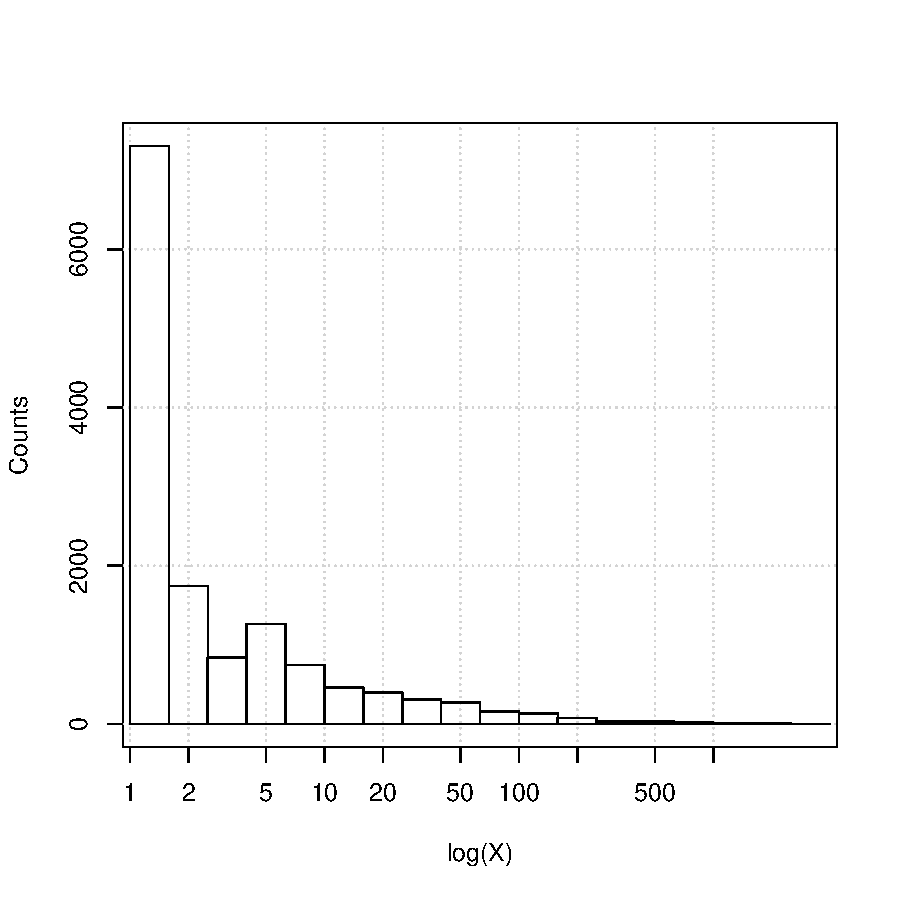
\includegraphics[width=0.5\textwidth]{sweave/sweave-lda-words-all-hist}
\label{fig:lda-words-all-hist}}
\subfloat[Subfigure 2 list of figures text][words with a frequency between 3 and 100]{
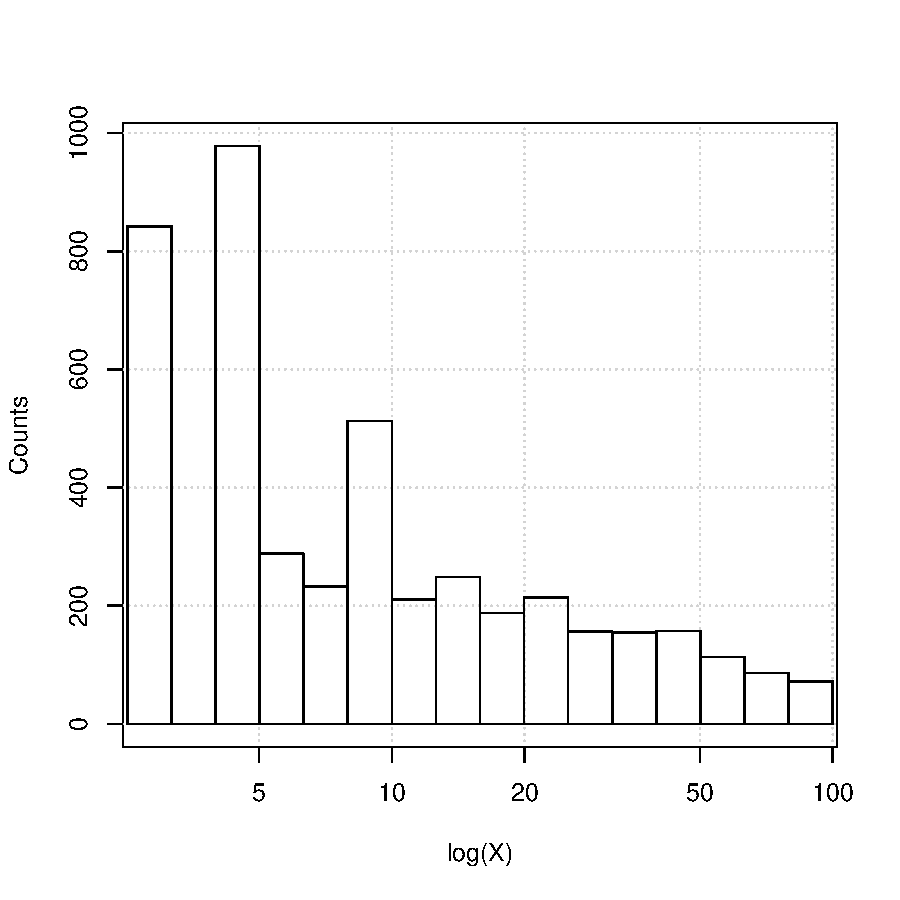
\includegraphics[width=0.5\textwidth]{sweave/sweave-lda-words-3-100-hist}
\label{fig:lda-words-3-100-hist}}
\qquad
\caption{Log-histogram for the words frequencies}    
\label{fig:lda-words-hist}
\end{center}
\end{figure}

I have manually checked the topics resulted after running the LDA model on the review corpus and they look logically coherent. The classifier results can be seen in Figure \ref{fig:lda}, where only the results for the IR measure were plotted. IR10 refers to the measure applied for 10 topics, IR30 means 30 topics and so on.

\begin{figure}[ht]
\begin{center}
\subfloat[Subfigure 1 list of figures text][Precision]{
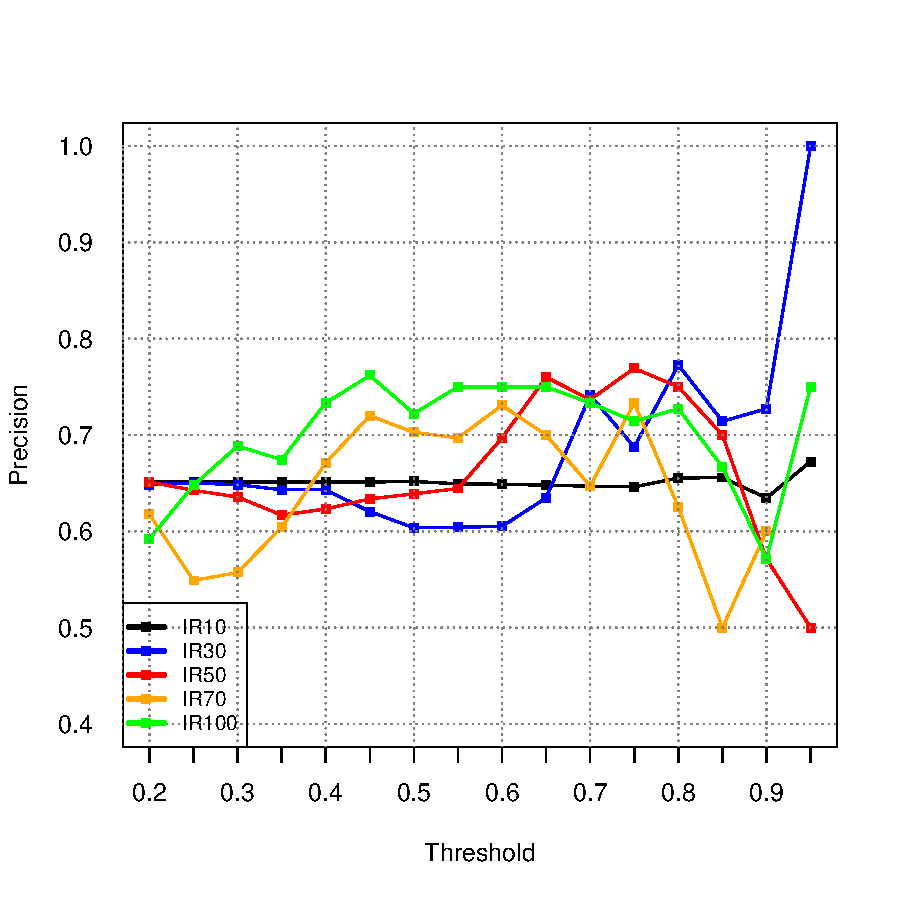
\includegraphics[width=0.5\textwidth]{sweave/sweave-lda-precision}
\label{fig:lda_precision}}
\subfloat[Subfigure 2 list of figures text][Recall]{
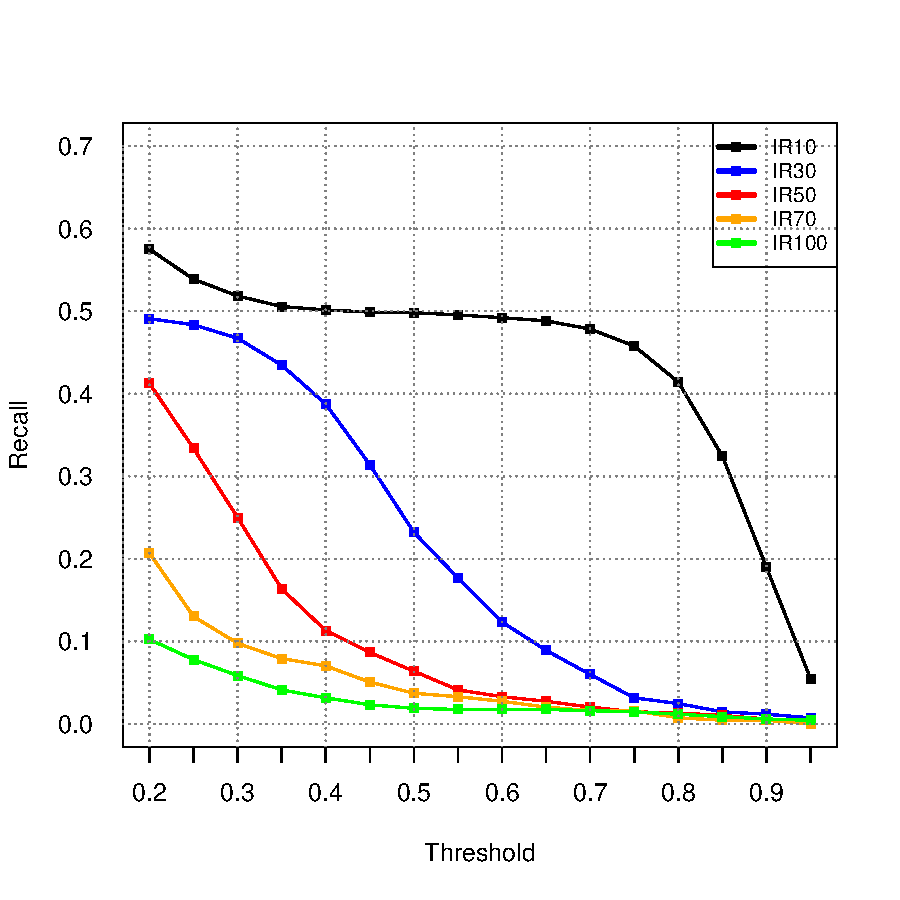
\includegraphics[width=0.5\textwidth]{sweave/sweave-lda-recall}
\label{fig:lda_recall}}
\qquad
\begin{center}
\subfloat[Subfigure 3 list of figures text][F1 Score]{
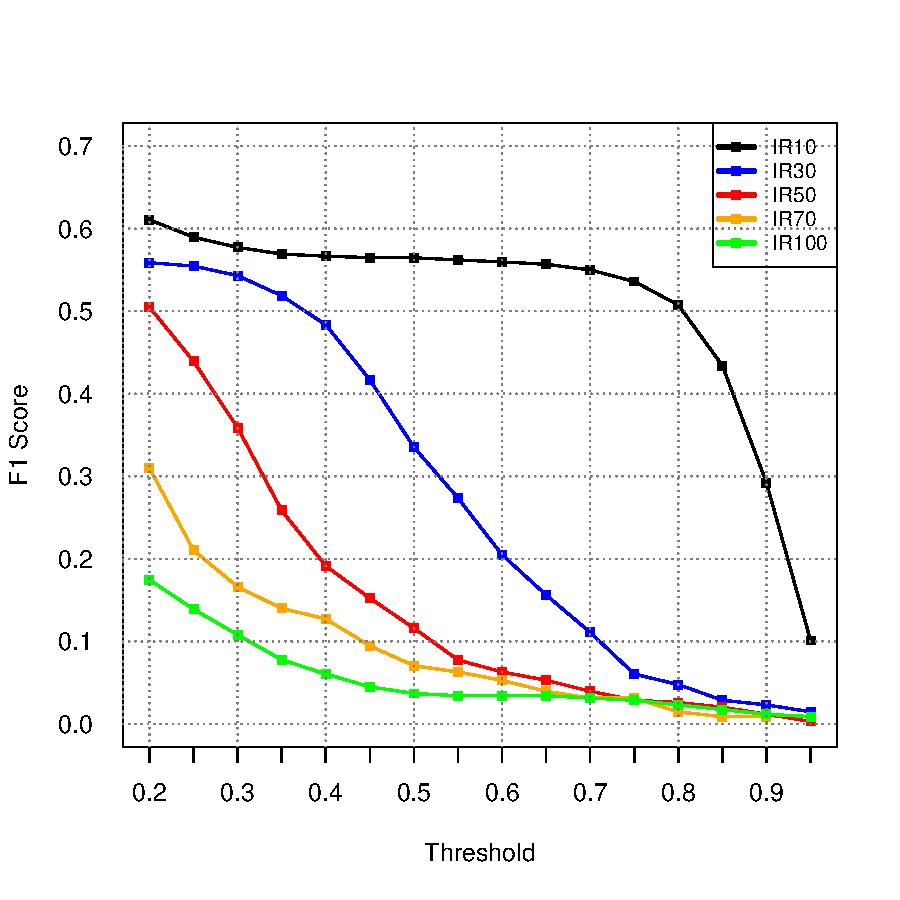
\includegraphics[width=0.5\textwidth]{sweave/sweave-lda-f1score}
\label{fig:lda_f1score}}
\end{center}
\caption{Classifier results for the information radius similarity measure}    
\label{fig:lda}
\end{center}
\end{figure}

\clearpage

Figure \ref{fig:lda_precision} shows the precision according to each value of the spam threshold. IR30 (IR measure for 30 topics) scored best and although the precision is not monotonic, generally it does not register significant drops as the threshold is increased. For thresholds of at least 0.7, it remains above 70\% and it peaks at 98\% for a 0.95 threshold. The model does not do so well for the other number of topics and registers significant drops in precision as the threshold is increased. 

The recall and F1 score values are consistent in relation to the number of topics. As the number of topics is increased, the model's performance decreases. The similarity results for 10 topics show the best F1 score, but the precision is more or less a flat line at 65\%. This could happen because 10 topics are way to little to summarize what people say about a seller. 

Table \ref{tab:lda} shows the precision, recall and F1 score of the classifier and the two gray lines indicate the threshold where both IR30 and IR50 scored best in terms of precision. The precision is lower but actually not far than that obtained using the semantic and vectorial similarity measures in the singleton opinion spam detection method, shown in Table \ref{tab:dbscan-minpts-2-eps-0-1-individual}. 

\begin{center}
% latex table generated in R 3.0.2 by xtable 1.7-3 package
% Tue Jul 01 18:39:50 2014
\begin{table}[!h]
\centering
\begin{tabular}{|l|l|l|l|l|l|l|l|l|l|}
  \hline
T & IR10 & IR10 & IR10 & IR30 & IR30 & IR30 & IR50 & IR50 & IR50 \\ 
  \hline
T & P & R & F & P & R & F & P & R & F \\ 
   \hline
0.2 & 0.65 & 0.58 & 0.61 & 0.65 & 0.49 & 0.56 & 0.65 & 0.41 & 0.51 \\ 
  0.25 & 0.65 & 0.54 & 0.59 & 0.65 & 0.48 & 0.55 & 0.64 & 0.33 & 0.44 \\ 
  0.30 & 0.65 & 0.52 & 0.58 & 0.65 & 0.47 & 0.54 & 0.64 & 0.25 & 0.36 \\ 
  0.35 & 0.65 & 0.51 & 0.57 & 0.64 & 0.43 & 0.52 & 0.62 & 0.16 & 0.26 \\ 
  0.40 & 0.65 & 0.50 & 0.57 & 0.64 & 0.39 & 0.48 & 0.62 & 0.11 & 0.19 \\ 
  0.45 & 0.65 & 0.50 & 0.56 & 0.62 & 0.31 & 0.42 & 0.63 & 0.09 & 0.15 \\ 
  0.50 & 0.65 & 0.50 & 0.56 & 0.60 & 0.23 & 0.34 & 0.64 & 0.06 & 0.12 \\ 
  0.55 & 0.65 & 0.50 & 0.56 & 0.60 & 0.18 & 0.27 & 0.64 & 0.04 & 0.08 \\ 
  0.60 & 0.65 & 0.49 & 0.56 & 0.61 & 0.12 & 0.20 & 0.70 & 0.03 & 0.06 \\ 
  0.65 & 0.65 & 0.49 & 0.56 & 0.63 & 0.09 & 0.16 & 0.76 & 0.03 & 0.05 \\ 
   \rowcolor[gray]{.7} 0.70 & 0.65 & 0.48 & 0.55 & 0.74 & 0.06 & 0.11 & 0.74 & 0.02 & 0.04 \\ 
  0.75 & 0.65 & 0.46 & 0.54 & 0.69 & 0.03 & 0.06 & 0.77 & 0.01 & 0.03 \\ 
   \rowcolor[gray]{.7} 0.80 & 0.66 & 0.41 & 0.51 & 0.77 & 0.02 & 0.05 & 0.75 & 0.01 & 0.03 \\ 
  0.85 & 0.66 & 0.32 & 0.43 & 0.71 & 0.01 & 0.03 & 0.70 & 0.01 & 0.02 \\ 
  0.90 & 0.63 & 0.19 & 0.29 & 0.73 & 0.01 & 0.02 & 0.57 & 0.01 & 0.01 \\ 
  0.95 & 0.67 & 0.05 & 0.10 & 1.00 & 0.01 & 0.01 & 0.50 & 0.00 & 0.00 \\ 
   \hline
\end{tabular}
\caption{Classifier results for LDA model} 
\label{tab:lda}
\end{table}\end{center}

Figure \ref{fig:lda-appendix-5-100-words} in the \nameref{chapter:Appendix} shows the classifier's performance when using words with a frequency between 5 and 100, having the log-histogram plotted in Figure \ref{fig:lda-words-hist-5-100-appendix}. Only reviews having at least 10 words after the word-frequency filtering step were considered. 
